\documentclass[11pt, a4paper]{article}

\usepackage{varioref}
\usepackage{hyperref}
\usepackage{cleveref}

\usepackage{listings}
\usepackage{subfigure}
\usepackage{graphicx}
\usepackage{titling}
% \usepackage[margin=1.8cm, includefoot]{geometry}

\usepackage{parskip}
\setlength{\parindent}{0cm}

\usepackage{titlesec}
\usepackage{pdfpages}

\usepackage{framed}

% Select what to do with todonotes:
% \usepackage[disable]{todonotes} % notes not showed
\usepackage[draft]{todonotes}   % notes showed

\newlength\longest
\interfootnotelinepenalty=10000
\titlespacing\section{0pt}{6pt plus 2pt minus 2pt}{0pt plus 0pt minus 2pt}
\titlespacing\subsection{0pt}{4pt plus 2pt minus 2pt}{0pt plus 0pt minus 2pt}
\newcommand{\subtitle}[1]{
  \posttitle{
    \par\end{center}
    \begin{center}\large#1\end{center}
    \vskip0.5em}
}

\setlength{\droptitle}{-4em}

\newcommand{\cmd}[1]{{\tt #1}}

\begin{document}

\title{Deeva}
\subtitle{A Java Debugger Suitable for Teaching}
\author{Kritaphat Sonsri-in, Xueqi Chen, Hector Dearman, \\Alina Draganescu, Felix de Souza}

\maketitle
\thispagestyle{empty} % No page numbers on first page.

% Report editing rules:
% Each sentence on a new line.
% Only edit one section before committing.
% Push after every commit.
% ONLY EDIT ONE SECTION BEFORE COMMITTING.

% Three main goals:
% 1. Fill a tool hole for first year Java course
% 2. Foster a strong mental model of imperative programming
% 3. Introduction to debugging

% Introduction
%   Set the scene (‘motivation’)
%   State the problem you are trying to solve (‘objective(s)’)
%   Summarise what you achieved (‘contributions’)
% Design & implementation
%   Detail your design (why did you do it this way?)
%   Summarise key implementation details (how did you do it? what tools did you use?)
% Evaluation
%   Summarise testing procedures (+ relevant testing results)
%   Evaluate your deliverables, e.g. in terms of performance, usability, usefulness…
%   (how successful was the project?)
% Conclusion and future extensions
%   Say what you’ve concluded from doing the work and how you’d build on it
% Project management
%   Planning, group organisation, breakdown + task allocation etc



\section*{Executive Summary}
\addcontentsline{toc}{section}{Executive Summary}

Deeva is a simple Java debugger for teaching which allows graphical introspection of a running program.

In the first year introductory Java course many students are encountering imperative programming for the first time so there is a strong desire to minimise `magic' particularly in the form of complex IDEs which `make it work'.
Unfortunately this attempt is hamstrung by the absence of a good Java debugger decoupled from an IDE.
Without a good strategy to fix broken programs students quickly reinvent bad habits ranging from the awful, shotgun debugging, to the merely poor, print statements.

What we want is a debugger, invokable from the command line, simple enough that students who have never seen a debugger before can taught to use it in only a few minutes but powerful enough to make tracking down a bug easy.
Deeva fills this hole in the Java ecosystem and Lab infrastructure.

Deeva was designed with an additional goal in mind.
At Imperial (as most places) students are taught imperative programming with diagrams, the lecturer draws a stack and a heap and shows how moving through the code effect the stack and the heap.
By using a novel user interface which resembles these diagrams we make debugging more intuitive, allow lectures to easily construct and step through these diagrams live on arbitrary code without fear of mistake and, for the first time, allow students to see how code they write is run on their own time without outside help.
This way Deeva becomes a tool for both teaching and learning.

All to many programmers, experts and beginners, never really learn to use or desire the powerful tools which already exist to introspect and modify running programs preferring instead to grovel though the source code with \cmd{printf}.
For students Deeva provides excellent introduction to these tools while also filling a vital gap in Lab infrastructure and providing a useful tool for lecturers teaching imperative programming.

% What is a debugger?
% ``Bugs'' are a type of software defect typically introduced though a mismatch between the programmers mental model of the system and the system itself.
% A ``debugger'' then is a program that allows programmers to inspect and manipulate the state and flow of a running system so they can understand the mismatch and hence fix the defect.

% Specifically students are encouraged to use a text editor and invoke the Java compiler and virtual machine directly in order develop a deeper and more transferable understanding of programming.
%
% first to help foster a strong mental model of imperative programming and secondly to introduce students to powerful introspection of software systems.

%the Imperial Computing department attaches great importance to practical programming ability much of students first year is spent learning several programming languages and completing many Labs, small programming tasks.
%The practical teaching of programming on the first year follows this progression: Functional programing, Imperative programing, Object Orientation and finally Systems programming.
%Historically the department has taught Functional programming using Haskell, OO programming using Java and Systems programming using C but for Imperative programing a few different approaches have been tried.

\clearpage
\tableofcontents
\clearpage

\section{Motivation}
\subsection{``Introduction to Imperative Programming" at Imperial}
Around half of first year undergraduate computing students at Imperial have no previous imperative programming experience\cite{projectproposal} so the course ``Introduction to Imperative Programming" run in the first term directly after ``Introduction to Functional Programming" forms a cornerstone of the practical education students receive giving them skills they will need in almost every other course.

The course focuses on the basics: control flow, functions and the write-compile-run cycle.
To make teaching more effective it is desirable to avoid introducing unnecessary complexity like Object Orientation, memory management or complex IDEs all of which are left to later courses.
For example, although the introductory course is now taught in Java it has previously been taught in Kenya\footnote{http://chatley.com/kenya/}, a language which acts as an imperative stepping stone to Java by allowing functions to exist outside of objects.

In particular, the department does not want students to end up relying on the large complex IDE like Eclipse or IntelliJ to `magically' run the code without understanding what it does.
So for the last two years students have been encouraged to avoid IDEs and instead use a text editor (like \cmd{vim}, \cmd{emacs} or \cmd{gedit}) and invoke the Java compiler (\cmd{javac}) and virtual machine (\cmd{java}) directly.
Unfortunately there is a downside to this approach, as most Java debuggers are integrated into IDEs and those which are not are often of poor quality. This coupled with the relatively complex UI of debuggers in general (see our analysis below) means that there is no good option for instructors to suggest to their class.
Students quickly encounter bugs in their programs and without a strong understanding of the language or a strategy to deal with bugs they are reduced to reinventing well known bad habits including an abundance of print statements, large try-catch blocks, making everything public or the plain wait for a miracle.

To combat this problem Dr. Tristan Allwood proposed\cite{projectproposal} this third year group project to build a tool to fill this gap.
A debugger which was: independent from an IDE, simple enough to be used by beginners but powerful enough to be useful.

%%The project also had another goal which was to be a tool for teaching.
Another main goal for this project is to be a teaching tool.
``Introduction to Imperative Programming" teaches fundamentals including control flow and the effect of assignment and function calls, return statements, etc
\footnote{A strong mental model of programming fundamentals is very important, for example when learning to program an early, consistent grasp of assignment is predictive of eventual achievement\cite{saeed09}.}.
As in many courses this is done diagrammatically, by showing how each line of code in a program effects the stack and heap.

\begin{figure}[h!]
\centering
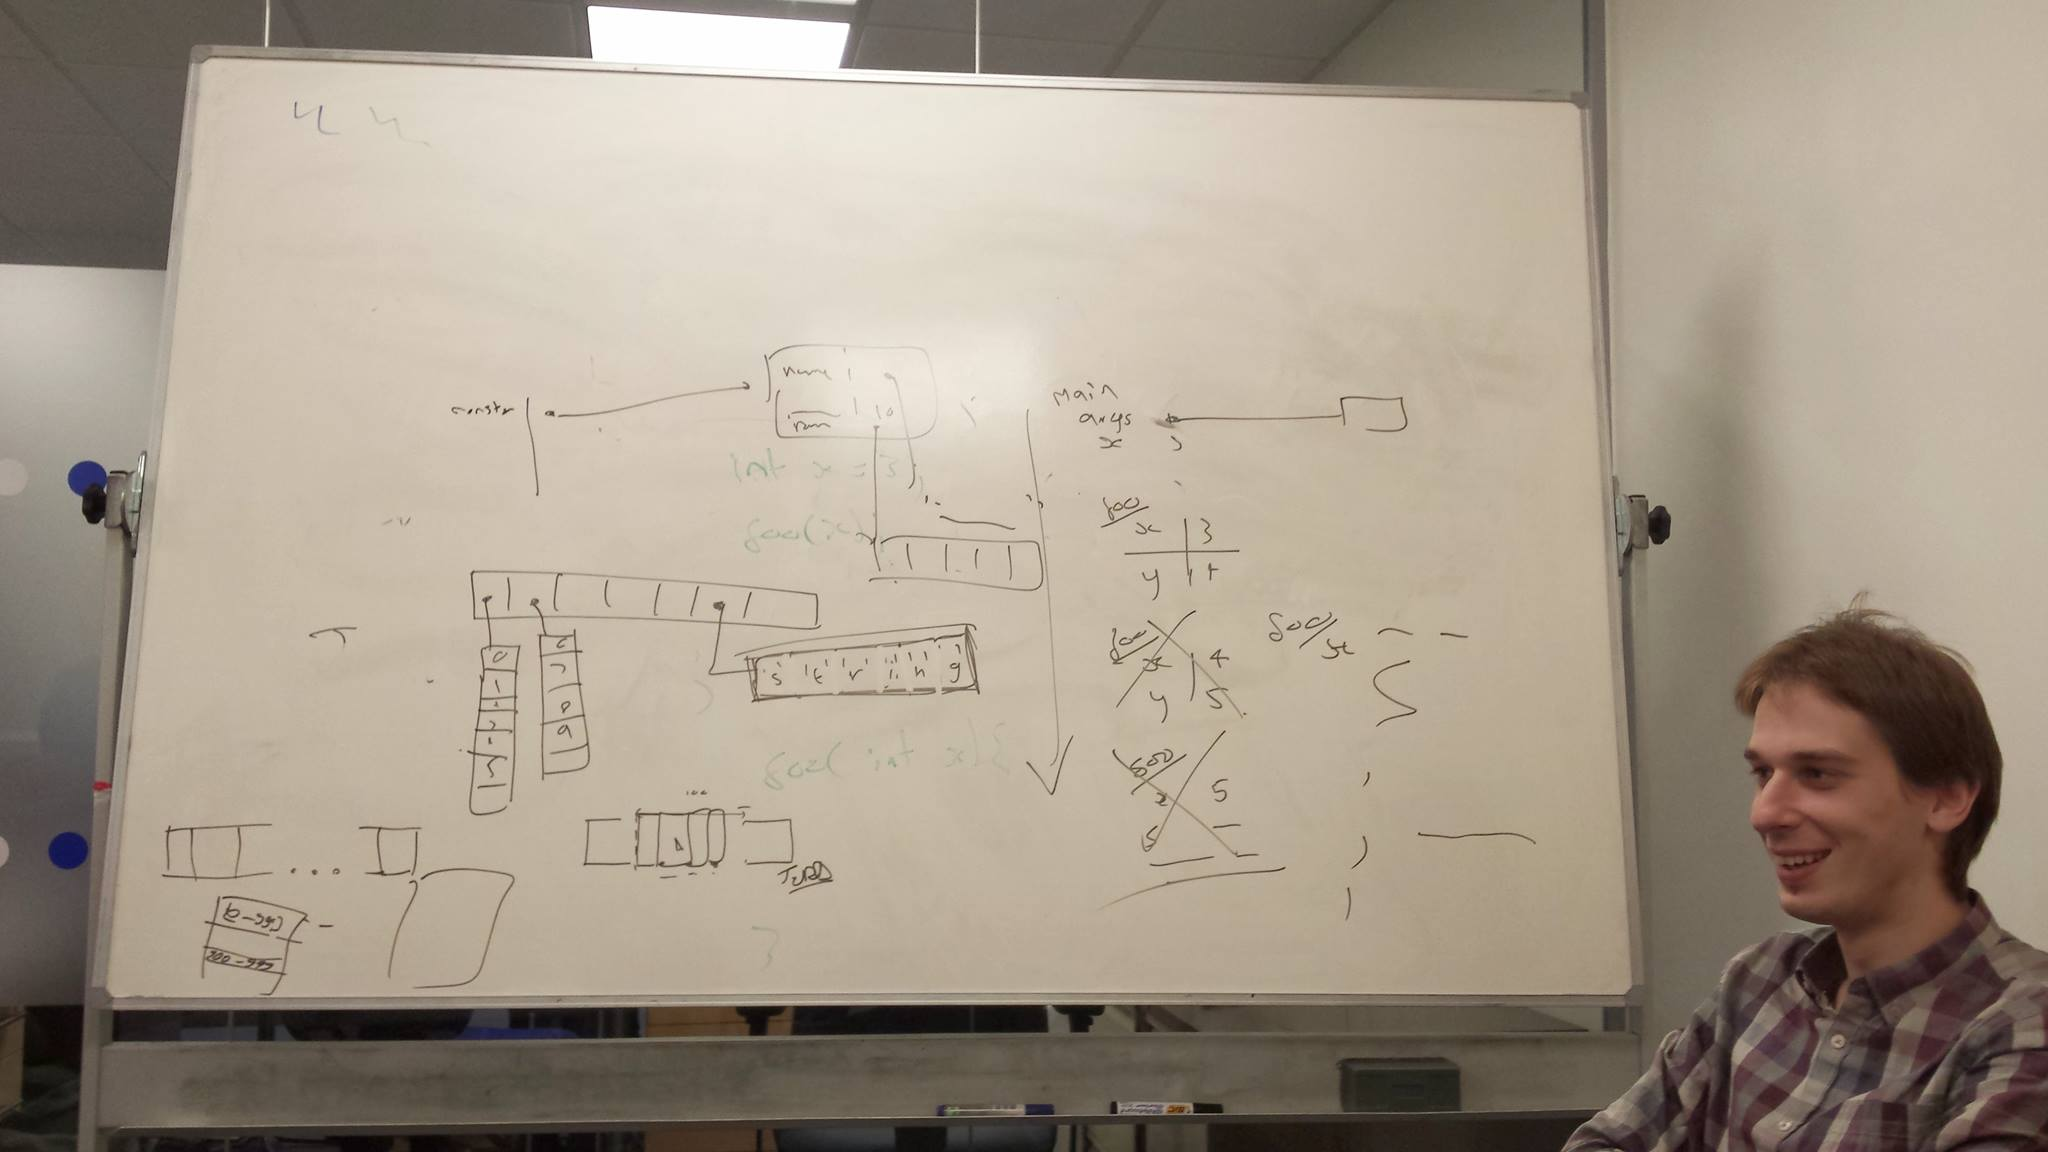
\includegraphics[width=125mm]{whiteBoardDrawing.jpg}
\caption{Example diagram of Stack and Heap}
\label{boarddiagrams}
\end{figure}

However this approach is not ideal.
It is time consuming and error prone to update the diagram and worse, it requires an oracle, the instructor, to act as mechanical interpreter of the rules.
Students have no way of graphically visualise the state of the programs they write, no easy way to see why their code does not have the effect they expect without ad-hoc experimentation: modifying the source code and hoping it exposes the original problem.

Some computer tools like \cmd{Python Tutor} \cite{pythontutor} are very useful at rendering a correct visualisation of the execution trace base on a code snippet.

\begin{figure}[h!]
\centering
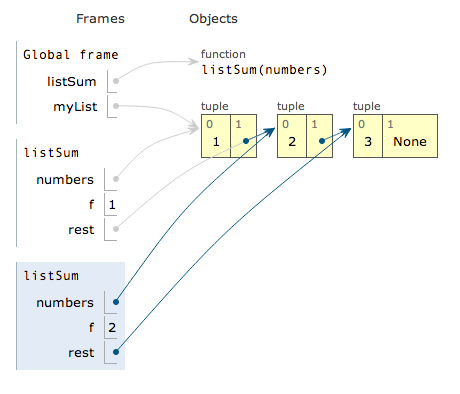
\includegraphics[width=125mm]{PythonTutorStackHeap.png}
\caption{Python Tutor Stack and Heap Diagram}
\end{figure}

By replacing the unintuitive tabular representation of the stack and heap found in almost every debugger with a user interface (based on these diagrams - see Figure \ref{boarddiagrams}) we hope to make Deeva a useful tool for teaching,
allowing instructors to create traces for programs in real time without making a mistake.
Even more importantly, it lets Deeva become a tool for learning, allowing students to explore the unfamiliar model of imperative programming without expert oversight.

Finally, despite the existence of powerful tools to introspect running programs many programmers continue to debug code using print statements.
This is probably due to the fact that they were not properly introduced to debugging tools or they found them too difficult to understand. So, with Deeva we are hoping to `inspire' new programmers to embrace debugging tools and to use them not only  for fixing bugs but also for understanding the workings of\texttt{•} different programming languages.

\subsection{Alternatives}
As part of our analysis stage, we looked at various different debuggers in order to decide what features we would like to include in Deeva. Our main interest was to find features that appeal to first year students (e.g. graphical visualisation) but does not overcomplicate the tool (e.g. watchpoints).
Below is a summary of our conclusions.

\subsubsection{jdb}
\begin{figure}[h!]
\centering
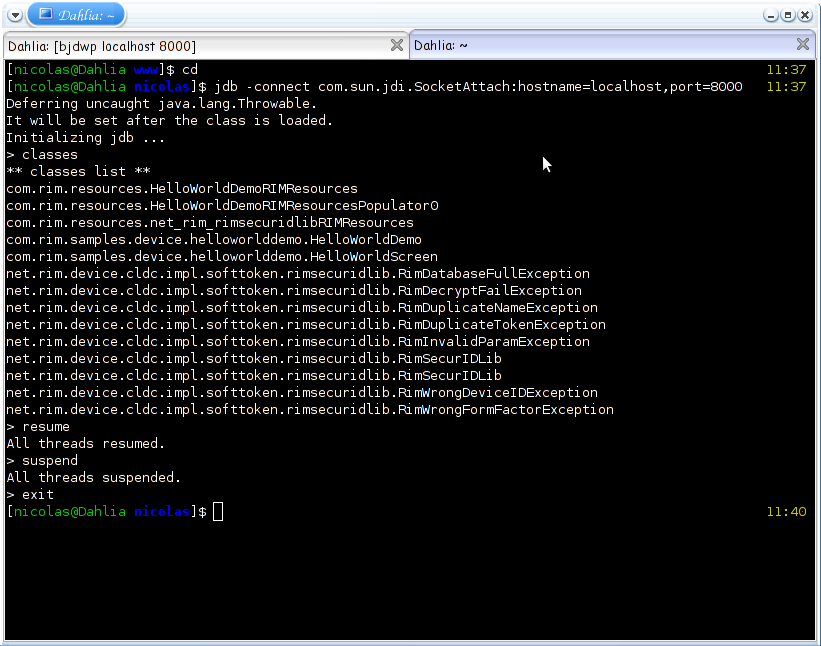
\includegraphics[width=125mm]{jdb.png}
\caption{jdb Debugger Screenshot}
\end{figure}

The Java Debugger, jdb, is a simple command line debugger that provides inspection and debugging for Java classes.
It provides most of the basic functionalities of a debugger eg. setting breakpoint(s), stepping through the next line, and diagnosing the cause of the exception.
However, since it is a command line debugger, it provides a poor graphic user interface.

Hence, jdb has the core functionalities we are looking for in a debugger but it is not supported by a good graphic representation. This makes it unintuitive for first year students, introducing the exact problem we are trying to solve.
\subsubsection{JSwat}
\begin{figure}[h!]
\centering
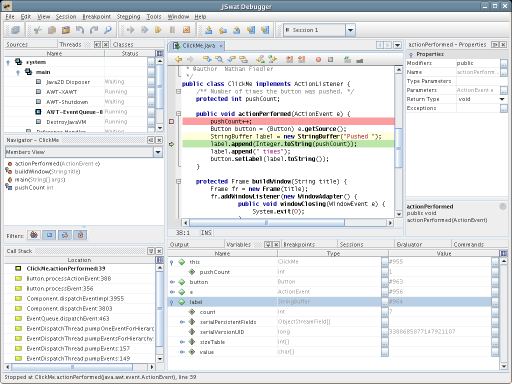
\includegraphics[width=125mm]{jswat.png}
\caption{JSwat Screenshot}
\end{figure}

JSwat is a graphical Java debugger which provides basic functionality like: setting breakpoints, thread and stack display, variable monitoring and method invocation.
The advantage of this tool (which is missing in most debuggers) is that it allows users to nicely `walk' through a linked list just by repeatedly clicking on a certain button.
Another benefit is its small size in terms of the disc usage.
However, its unattractive interface with a multitude of features might still overwhelm a debugging beginner.

Finally, JSwat is a tool that is closer to what we are trying to achieve but we found that it is still too complicated for our purposes.

\subsubsection{Eclipse Debugger}
\begin{figure}[h!]
\centering
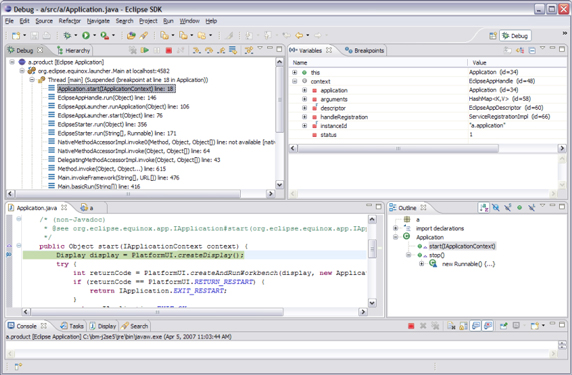
\includegraphics[width=125mm]{eclipse.jpg}
\caption{Eclipse Debugger Screenshot}
\end{figure}

Eclipse allows the user to start a Java program in Debug mode which provides a control of the execution process and allows for investigation of the variable state.
In addition, it provides a lot more functionalities than jdb, such as setting conditional breakpoints, modifying variables, friendlier graphic user interface etc.
Nevertheless, Eclipse is an integrated IDE debugger that has a lot of features that beginner will not use.

In concluion, although Eclipse is one of the most used and reliable IDEs it is not suitable for beginners as it wraps debugging in a `magical' black box which is exactly what the lecturers are trying to avoid.

\subsubsection{IntelliJ Debugger}
\begin{figure}[h!]
\centering
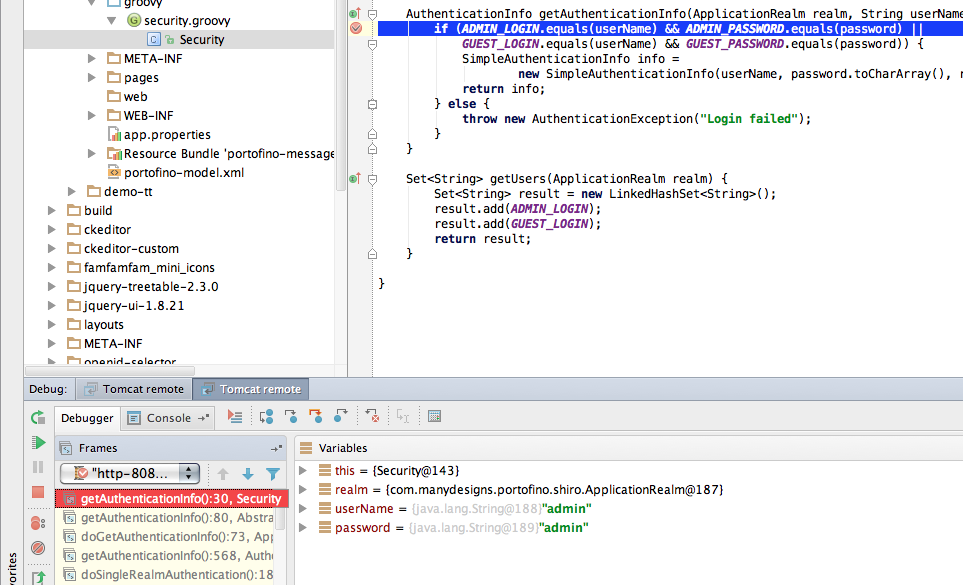
\includegraphics[width=125mm]{intellij.png}
\caption{IntelliJ Debugger Screenshot}
\end{figure}

Similar to Eclipse Debugger, IntelliJ Debugger is also an integrated IDE debugger which provides fast and powerful functionalities.
Even though it also provides nice features that allow for easy object inspection, it is again overwhelming first year students.
\subsubsection{Python Tutor}
\begin{figure}[h!]
\centering
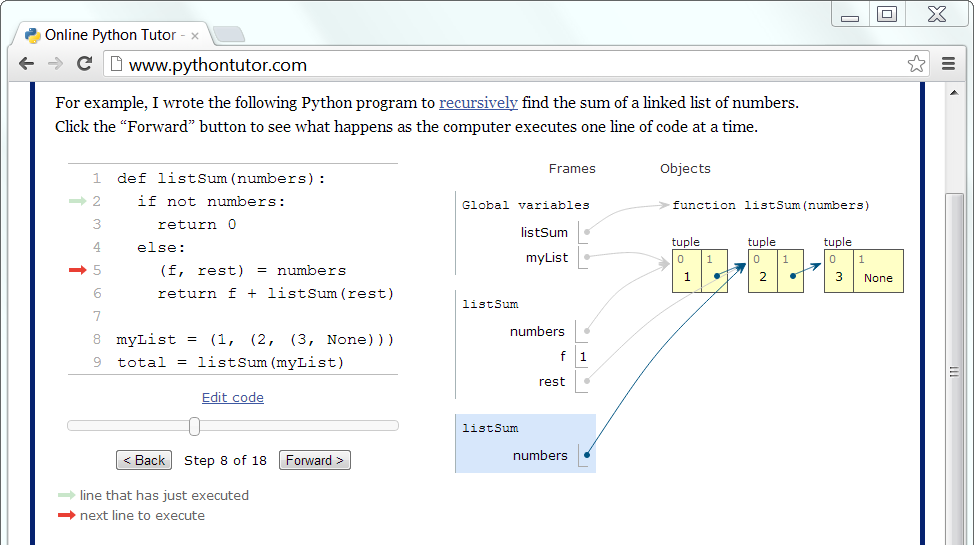
\includegraphics[width=125mm]{pythontutor.png}
\caption{Python Tutor Screenshot}
\end{figure}

Python Tutor is not a debugger but an online tool that provides users with a visualisation of the program state.
A user can write a Python program in the web browser and visualise what happens as each line of the code gets executed.
It can play through the program trace forwards and backwards, a functionality that is absent in most debuggers.
This would be a very useful tool for first year students except that it uses Python not Java. Also, it does not support classical debugger movement (e.g. step in, step into), user input or multiple files.

However, it does have a much better way of displaying the state of the program, making the program execution very easy to understand. This feature appealed a lot to us as we wanted to make it the selling point of Deeva.


\section{Objectives}

Our objective was to produce a Java debugger that was:

\begin{description}
\item[Independent] \hfill \\
The debugger is a separate tool started from the command line, it does not require or run inside a IDE.
\item[Powerful] \hfill \\
The debugger is powerful enough to solve real problems.
\item[Simple] \hfill \\
The debugger is intuitive enough to be easily picked up by first year students.
\end{description}

At the start of the project we produced a initial plan (for the full plan please see ~\cref{sec:initialplan}) where we broke these high level objectives down into a minimal set of concrete goals which we then had signed off by Dr. Allwood.

\begin{itemize}
\item Must run in the Labs
\item Start from the command line
\item Supporting all the command line switches (-ea etc)
\item Taking command line arguments (from the gui)
\item Users must be able to see stdin, stdout, stderr
\item Users must be able to see the source code
\item Users must be able to inspect the current state of the program somehow
\item Run/Pause/Step into/Step Over
\item Multiple Files
\item Breakpoints
\item Supports Java static methods, Objects, Arrays, Control flows, Generics, Enumerations
\item Minimal Documentation (--help, README, small user guide, etc)
\end{itemize}

Similarly we produced a prioritised list of extensions:

\begin{enumerate}
\item Lecture Mode
\item Display of state is graphical
\item Pictures of previous state and current state for comparison
\item Conditional breakpoints
\item Watch points
\item Multi-platform (OSX, Linux, Windows)
\item Maximal Documentation
\item Support all of Java features (Threads etc)
\end{enumerate}

\section{Deeva}
\subsection{Starting the program}
\subsection{Run}
\subsection{Breakpoints}
\subsection{Next/Into/Out}
\subsection{Warning about uncompiled programs.}
\begin{figure}[h!]
\centering
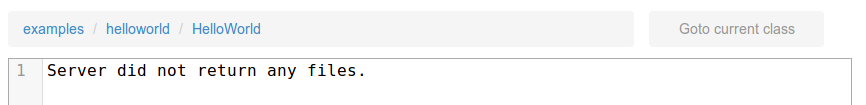
\includegraphics[scale=0.6]{warningFeature.png}
\caption{Warning about Uncompiled Programs Screenshot}
\label{fig:warningFeature}
\end{figure}

\subsection{Stack Heap}
\subsection{Expansion}
\subsection{Arguments}
\begin{figure}[h!]
\centering
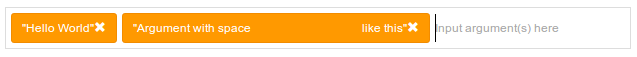
\includegraphics[scale=0.7]{argumentFeature.png}
\caption{Arguments Feature Screenshot}
\label{fig:argumentFeature}
\end{figure}
\subsection{Assertion}
\begin{figure}[h!]
\centering
\subfigure[Assertions Disabled]{
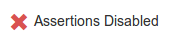
\includegraphics{falseAssertionFeature.png}}
\quad
\subfigure[Assertions Enabled]{
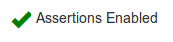
\includegraphics{trueAssertionFeature.png}
\label{fig:argumentFeature}}
\caption{Different states of Assertions}
\end{figure}

\subsection{Stdin/Stdout/Stderr}
\subsection{Stop}
\subsection{Current State}
\begin{figure}[h!]
\centering
\subfigure[Current State is ``Program not running"]{
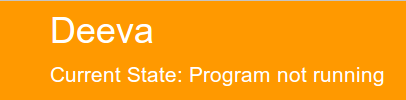
\includegraphics[scale=0.5]{notRunningCurrentStateFeature.png}}
\quad
\subfigure[Current State is ``Program paused"]{

\includegraphics[scale=0.5]{pausedCurrentStateFeature.png}
\label{fig:argumentFeature}}
\caption{Different states of Current State}
\end{figure}

\subsection{Multiple Files}
\begin{figure}[h!]
\centering
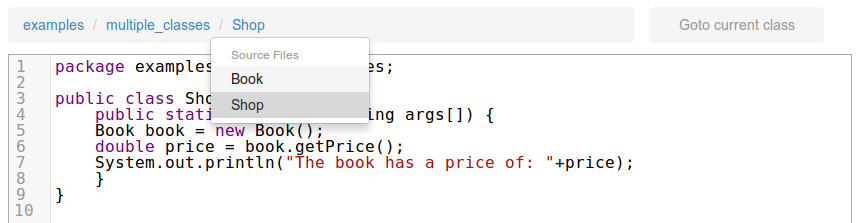
\includegraphics[scale=0.5]{multipleFileFeature.png}
\caption{Multiple Files Feature Screenshot}
\label{fig:multipleFile}
\end{figure}

\subsection{Server Quit}
\begin{figure}[h!]
\centering
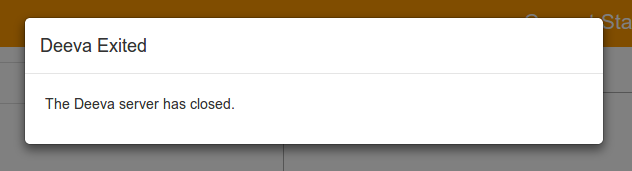
\includegraphics[scale=0.6]{exitFeature.png}
\caption{Server Quit Screenshot}
\label{fig:quitFeature}
\end{figure}

\subsection{Deeva in the Labs}
\todo{??}
\section{Design}

After the project assignment, we had our first meeting with Tristan in order to disscuss his expectations for the debugging tool along with our ideas about the project requirements.

We found that Tristan's motivation behind setting such a project was to have a teaching tool that can graphically represent the state of Java programs. In lectures, he uses the whiteboard to create a picture of the stack and the heap at different points in the program like you can see in Figure \ref{fig:sketch}. However, he wanted a debugger suitable for teaching with a graphical representation as the whiteboard method is time consuming and offers less consitency than a automated tool.
Therefore, we decided to use his whiteboard sketches as the starting point for Deeva's user interface, mostly because we found his drawings intuitive and accurate.

\begin{figure}[h!]
\centering
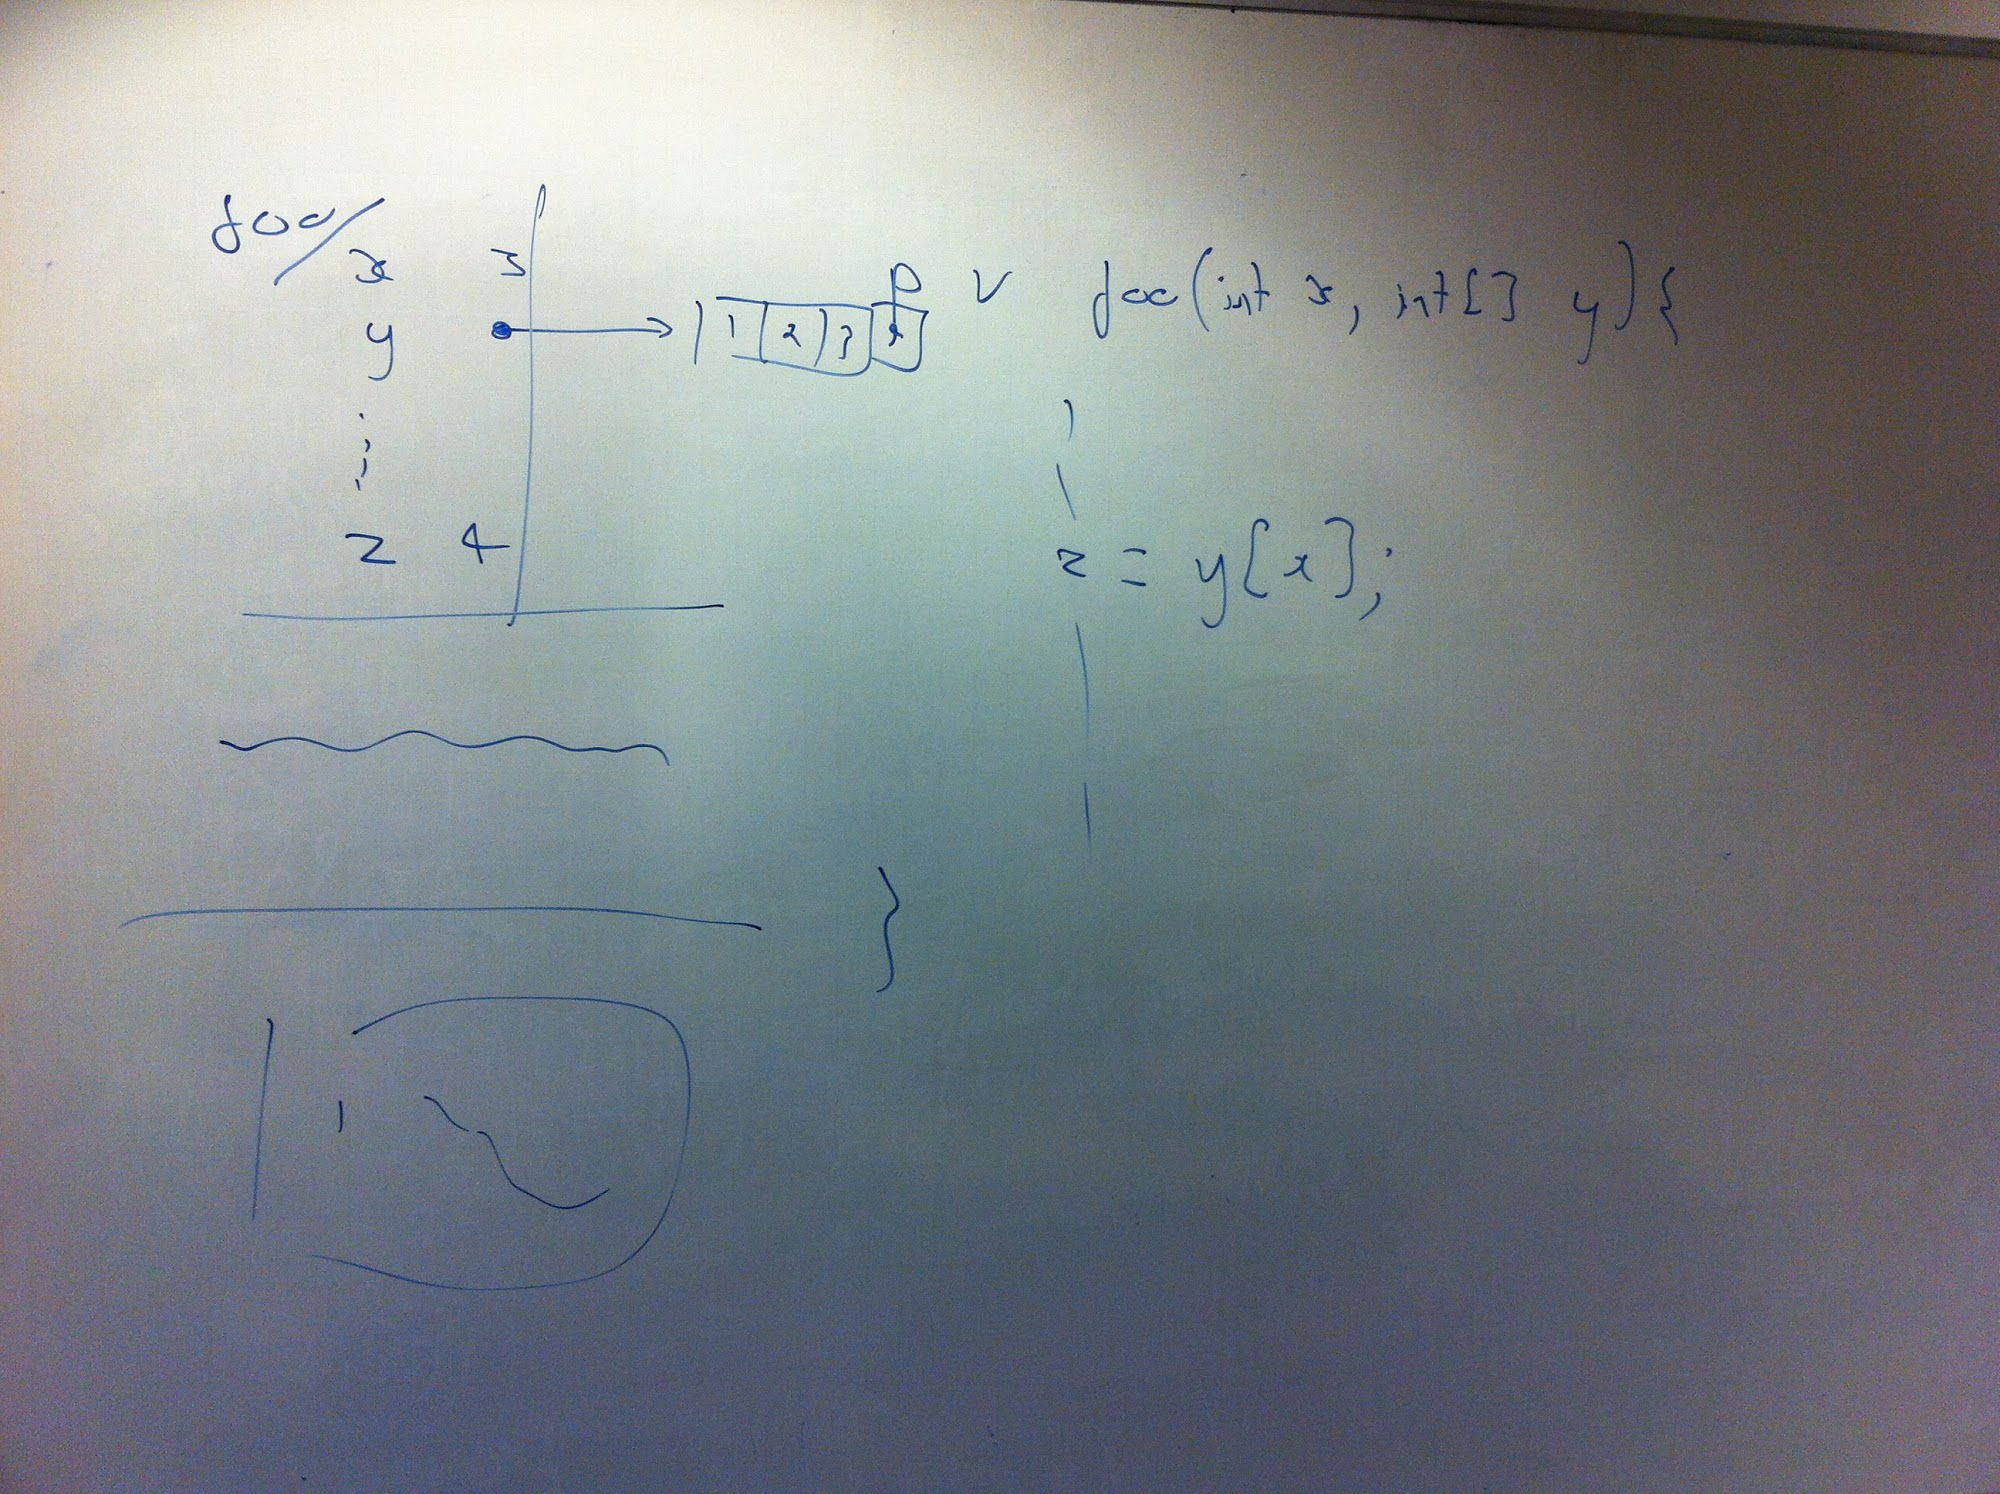
\includegraphics[width=\textwidth]{sketch.jpg}
\caption{Tristan's whiteboard representation of a Java program}
\label{fig:sketch}
\end{figure}

To avoid the costly mistake of spending a lot of time designing and building a UI that we may not use for the final product we decided to create a mocked front end design that satisfies both our and Tristan's requirements. We acheived this by disscussing differnet approaches with Tristan, sketching them on the whteboard and the transposing the idea in a Google Doc mockup (Figure~\ref{fig:mockup}).

\begin{figure}[h!]
\centering
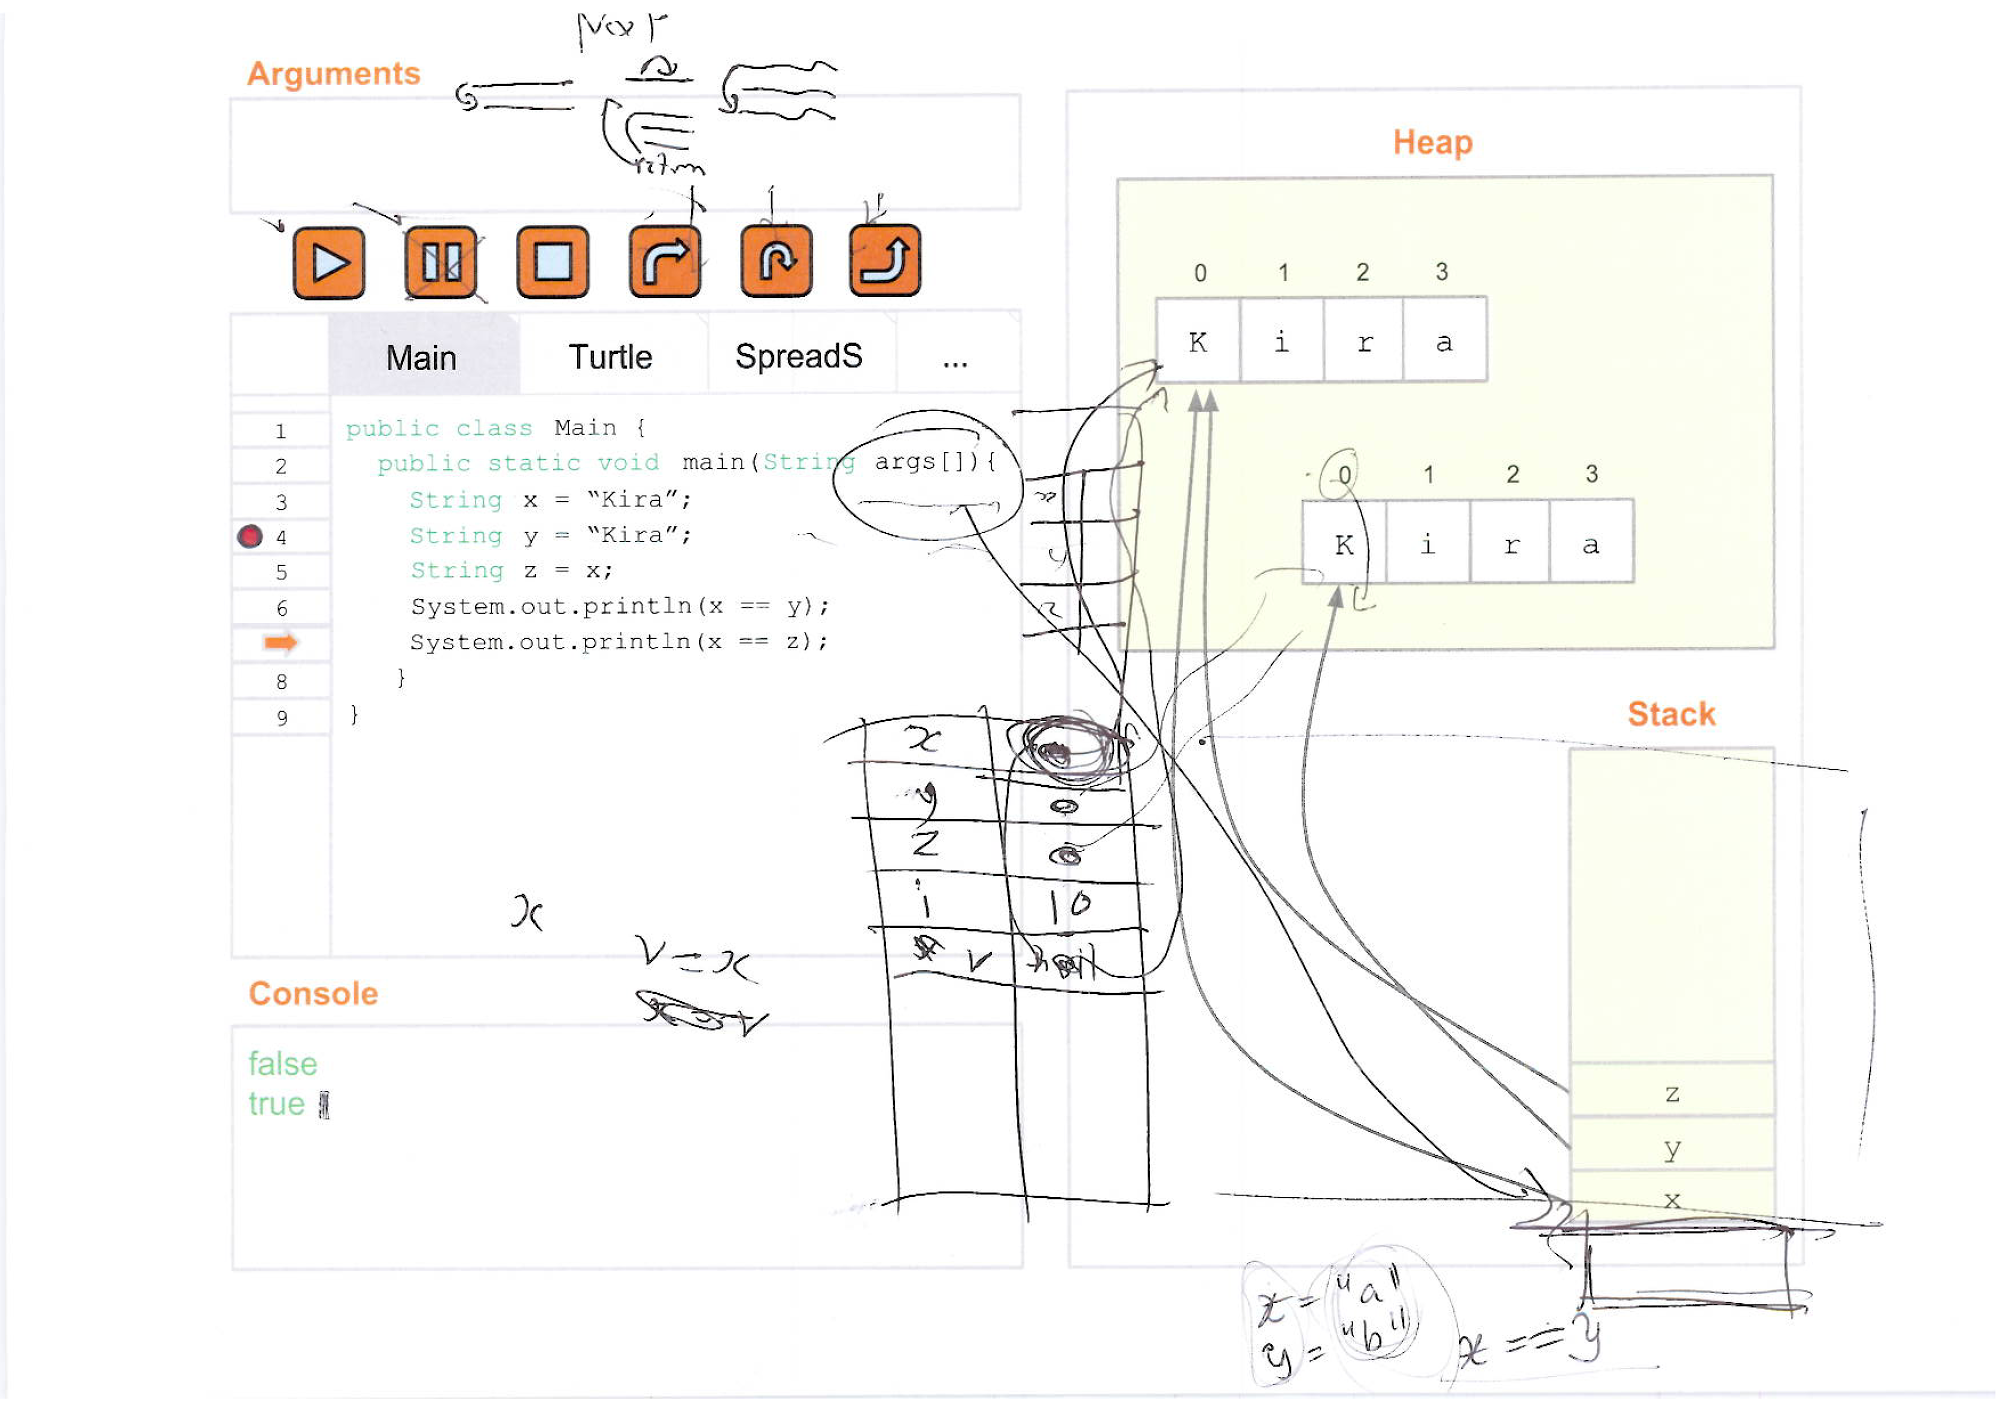
\includegraphics[width=\textwidth]{mockup.png}
\caption{Mocked up example}
\label{fig:mockup}
\end{figure}

This approach also made it easy to modify the design and to ask for feedback from first year students.
However, this strategy did not solve every problem.
For example, we completed a UI version that was generally agreed to be a good design on paper but had flaws (e.g. not readable from the back) that were discovered once we tried it on the screens in one of the lecture rooms.
As a result, we decided to test our mockups on the lecture room screens after each major design change to minimise the chance of unexpected issues once the UI has been implemented.

\subsection{Frontend Design}
\subsubsection{Overview}

Each component of the user interface was built to represents core features of the project, like the ability to view the source code or the possibility of reading from \texttt{stdin}.

The UI is esentially divided into two large parts.
On the left hand side there is a tab-like bar that enables the user to easily add or remove program arguments, a series of buttons representing the main debugging actions (run, stop, next, step into, step out), a dropw-down list that displays all the available classes from the package that could be loaded in the code pane and finally the code pane that displays the source code or the previously selected class.

On the right hand side there is a console input/output area that allows for comunication with \texttt{stdin}, \texttt{stdout} and \texttt{stderr}. The rest of the space is filled by the graphical representation of the current stack and heap state.

\subsubsection{UI Design}
\begin{figure}[h!]
\centering
\subfigure[First UI Design]{%
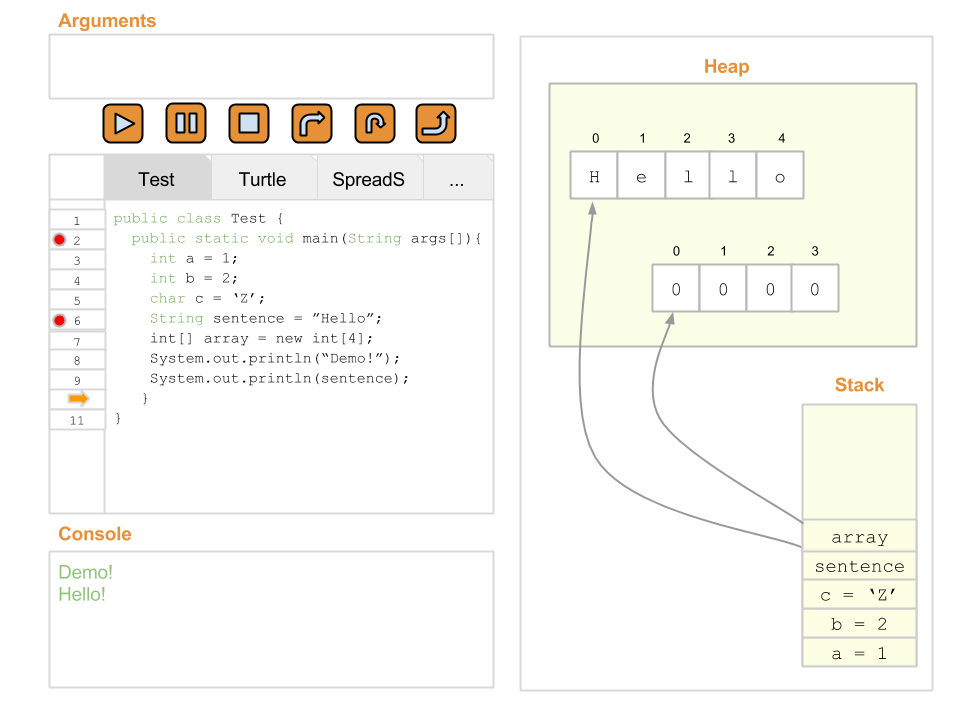
\includegraphics[height=70mm, width=60mm]{designIdea1.png}}
\quad
\subfigure[Second UI Design]{%
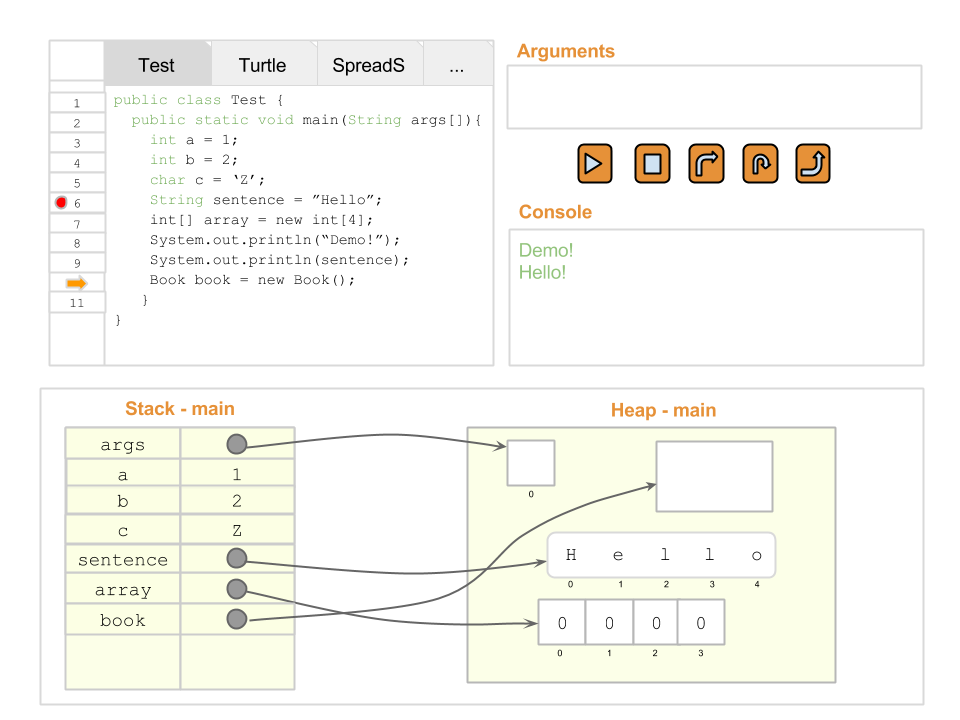
\includegraphics[height=70mm, width=60mm]{designIdea2.png}
\label{fig:designIdea2}}
\caption{Different views of the UI designs}
\end{figure}

Initially, we considered a few different posibilities for the UI design in order to find the one that would be most suitable for regular use. We considered the pros and cons of all of them before deciding on the final design version. Here are some of the ideas we considered:

After discussing with Tristan, we thought that if we put the stack and the heap visual at the bottom of the page we could better manage scenarios like small screens, a large heap and large arrays.
As a result, we modified our UI design to be similar to the figure~\ref{fig:designIdea2}.\\
\begin{figure}[h!]
\centering
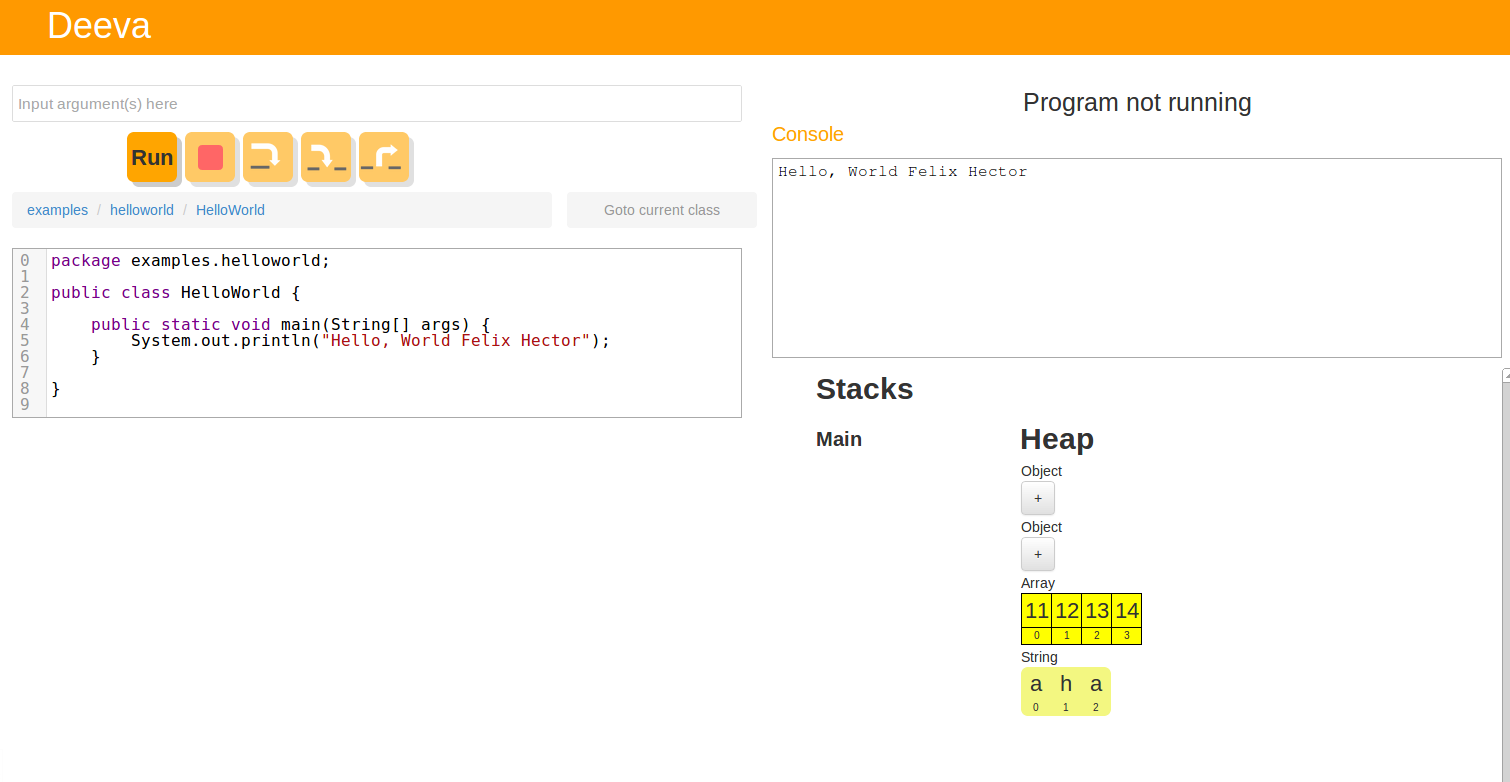
\includegraphics[height=70mm,width=130mm]{finalDesign.png}
\caption{Final UI Design}
\label{fig:finalDesign}
\end{figure}

However, we discovered that when the stack grows larger the user would need to scroll up and down between the source code and the graphical representation which we considered to be a major unconvenience when using Deeva regularly.
In order to solve this problem we considered making the code pane fixed to the top of the screen so it is visible even when scrolling.
This introduced other problems like the overlapping of the code and the graphic display.
Therefore, we agreed on putting the stack and heap on the right hand side with some modification to the initial design (see figure~\ref{fig:finalDesign}).

\subsubsection{Button Design}
The essential feature of any debugger is the ability of gradual navigation through the code by using combinations of the next, step in, step out and run actions.
Hence, the visual representation of these actions in the UI had to be carefully considered.
Using buttons was the natural choice for these actions. However, choosing the buttons' design required a detailed research to find out what would appeal to our main users, first year students.
After conducting a quick survey (see ~\cref{sec:evaluation}) on students from different years with both computing and non-computing backgrounds, we discovered that most people found the buttons names and designs in Eclipse to be very confusing.
As a result, we designed several different sets of buttons and used a questionnaire to pick among them.

\begin{figure}[h!]
\centering

\includegraphics[height=20mm,width=60mm]{buttons1.png}
\caption{Initial Design of the ``Stepping'' Buttons}
\label{fig:button1}
\end{figure}

Figure~\ref{fig:button1} shows our original design of the ``Stepping'' buttons.
They inherit the design from the Eclipse debugger.
They are \cmd{Step Into}, \cmd{Step Over} and \cmd{Step Return} from left to right respectively.

\begin{framed}
\emph{A digression on the behavior of the Stepping buttons.}
\todo{I don't know what exactly this box is supposed to mean.}
Given a program counter pointing
\begin{description}
\item Step Into
\item Step Over
\item Step Return
\end{description}

\end{framed}


We asked a friend who does not study Computing and has never used a debugger but had exposure to programming to guess which stepping action corresponds to which button for the Eclipse debugger.
He found it difficult to correctly match them just by the buttons' visual design, confirming our suspicion that these are not the most intuitive of designs.
We was then explained the concept of \cmd{Step Into}, \cmd{Step Over} and \cmd{Step Return} in terms of debugging. Asked again if he thought any of them really matched the buttons, he gave us some valuable feedback: ``It would be useful if we could somehow represent different scopes/lines so that the arrows (along with their direction) can correctly express the intended function.''
\begin{figure}[h!]
\centering

\includegraphics[height=20mm,width=60mm]{buttons2.png}
\caption{Redesign of the ``Stepping'' Buttons}
\label{fig:buttons2}
\end{figure}

Figure~\ref{fig:buttons2} represents our second design.
As suggested by our friend, the black lines indicate the lines of code which is similar to an editor.
Arrows going in either the upwards or downwards directions indicate going to the next line, function, or (or previous) scope.
We created a questionnaire in which we explained the definition of ``Next", ``Into" and ``Out" (our new and hopefully more intuitive names for the functionality previously known as ``Step Into'', ``Step Over'' and ``Step Return'').
\todo{section needs redesigning}
Then we asked which of the eight button designs best represents the aforementioned functions.
We gave out the questionnaires (see ~\cref{sec:buttonquestionnaire}) when we did the Hallway Testing (see ~\cref{sec:evaluation}) to some first year students and second year students.
Our second set of designs were much more popular than the original design among first year students.
However most of the second year students chose the original Eclipse design, one of them explaining that because they had already used Eclipse they were used to the original buttons.

In the end we did not use the second design because of some confusion from our users and comments from our project supervisor during the process.
It was not that clear what the black lines indicate especially for experienced users who are already used to the original design common to many debuggers additionally given that we expect users to graduate to using the Eclipse and other debuggers we did not want to create a whole new design vocabulary that they would soon have to relearn.
We did however keep the new more intuitive names.

\subsubsection{Colour Scheme and Font Size Design}
One of Deeva's desired feature that would set it apart from other debuggers is a nice interface that would appeal to all of our users.
As our two main stakholders are students using the tool themselves on the lab machine and students observing the lecturer using the tool on the lecture room screens, we had to cater for different visual requirements, including choosing the right color scheme and font design.

When choosing the color scheme we considered a set of diferent issues, for example, the colours should not be to tiring for the student that is using it for his personal use and is close to the screen, the color scheme has to be visible to all students including those with some form of visual impairment or the scheme used has to subconsciously keep the users interested.
Similarly, the font sizes had to be suitable for both stakeholders.

We carried out a questionnaire on the first year Java class to see which colour scheme and font size are the most liked and most visible on the projector in the lecture hall.

\begin{figure}[h!]
\centering
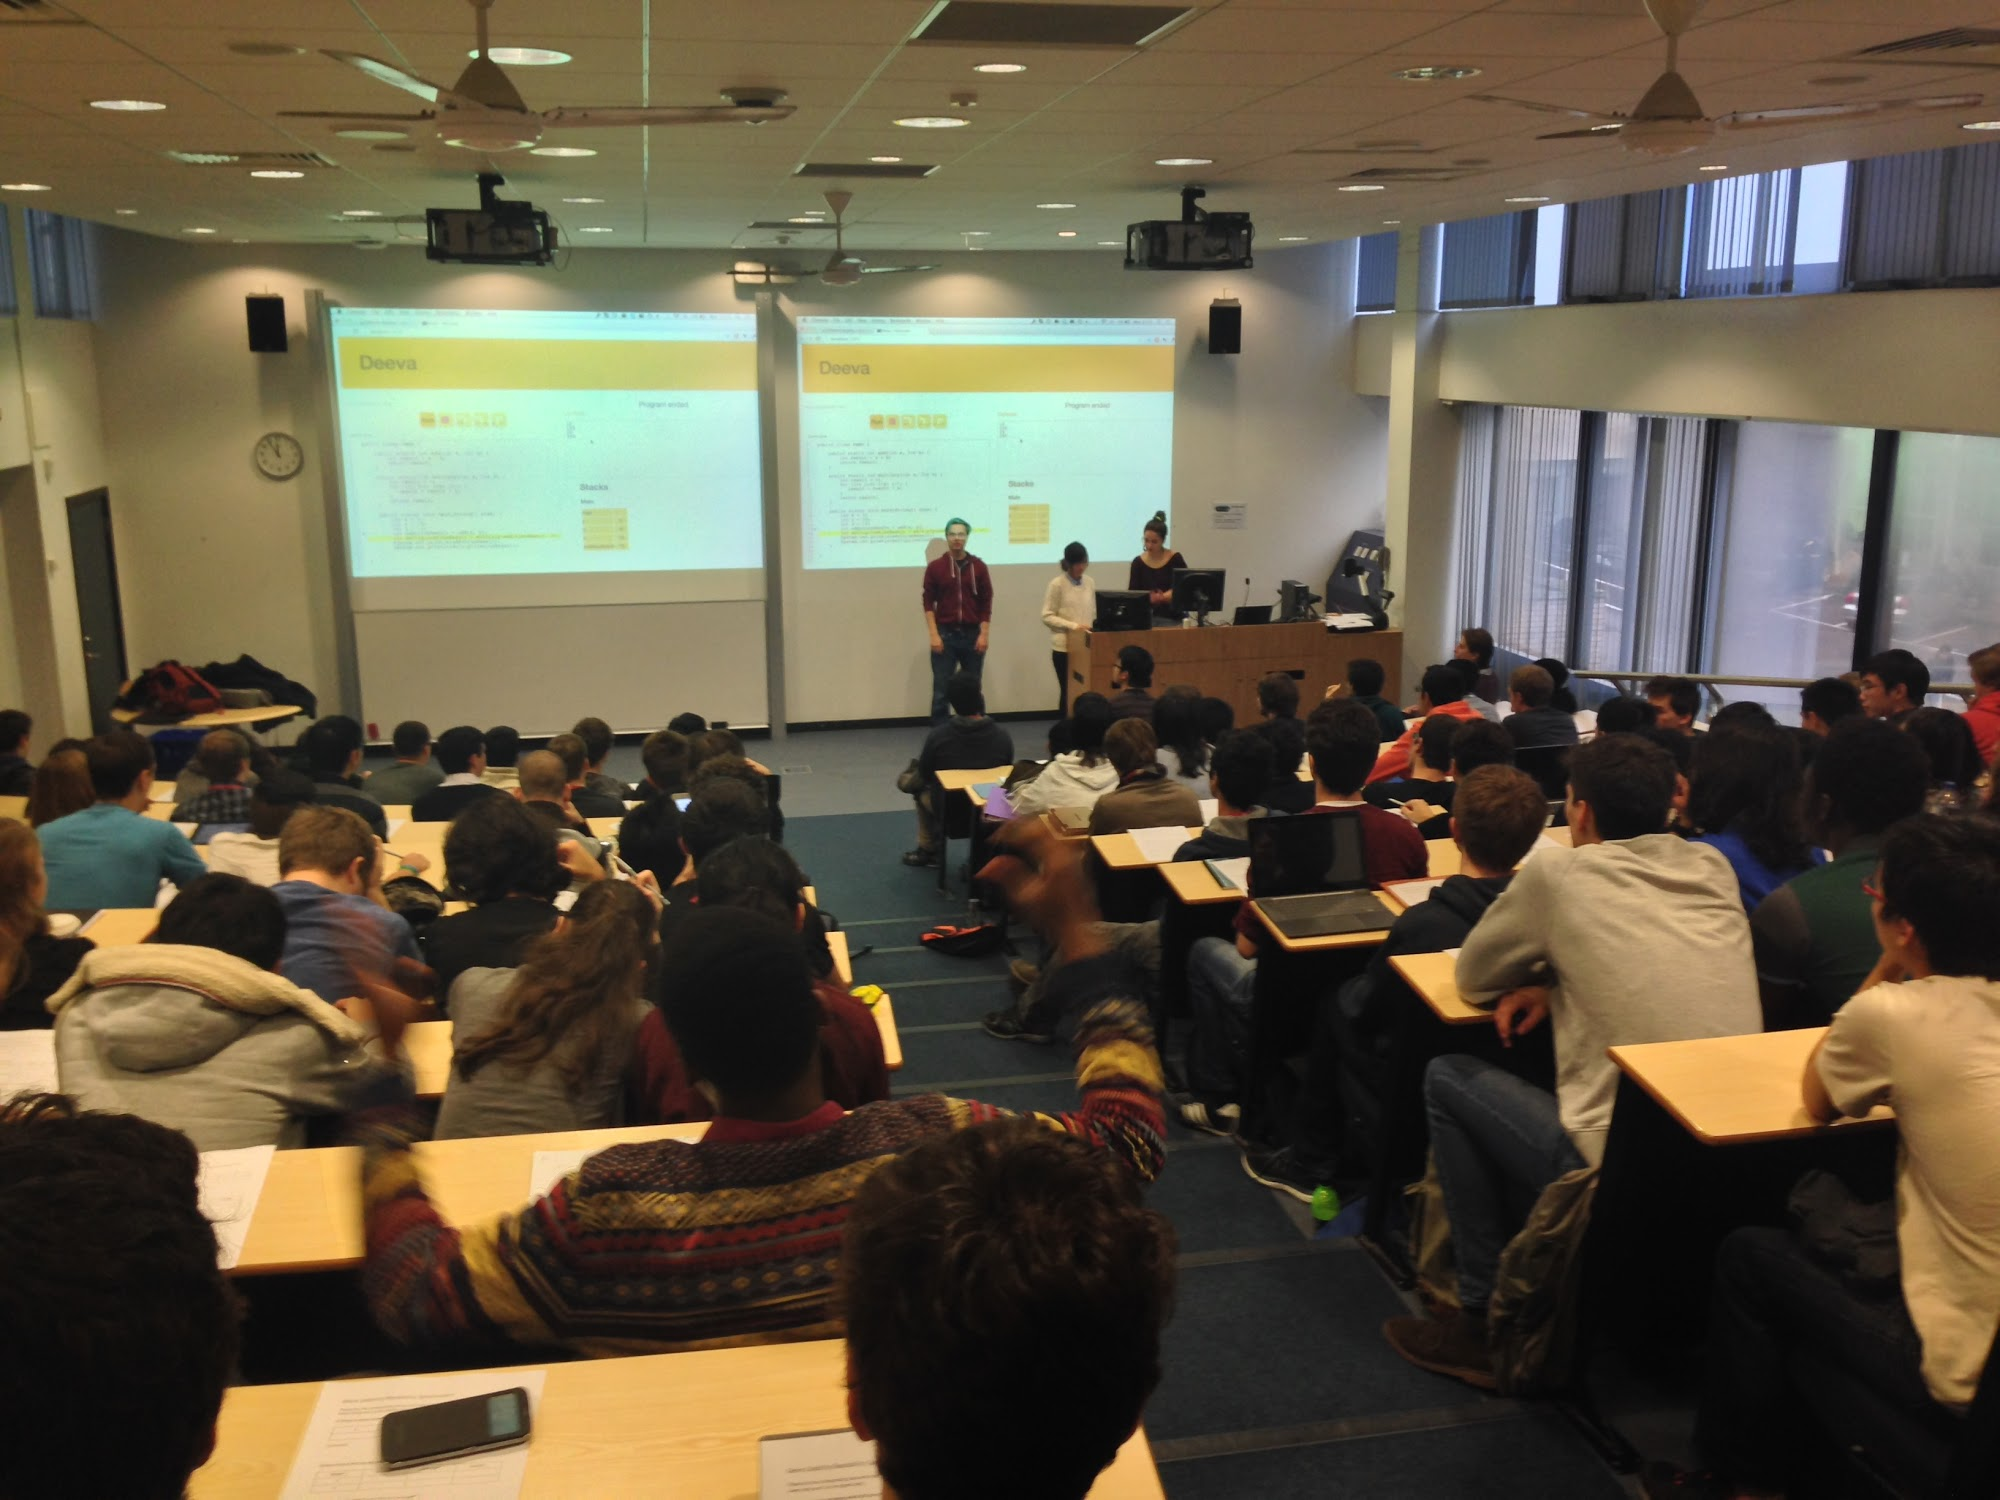
\includegraphics[height=50mm,width=100mm]{lectureHall.jpg}
\caption{Font size and colourscheme test in first year lecture.}
\end{figure}

Given 5 different colour schemes, the preferred choice was our current colour scheme (orange), followed by a light blue color scheme (see figure~\ref{fig:colours}).
This validated our initial research that showed that in visual presentations, people are attracted to bright, warm colours that express optimism.
\begin{figure}[h!]
\centering
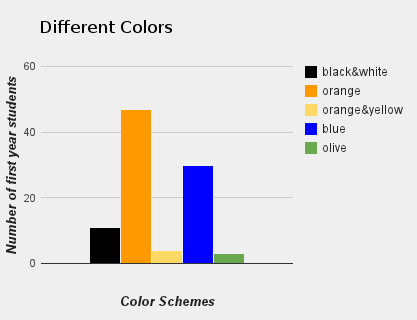
\includegraphics[height=60mm,width=100mm]{colours.png}
\caption{A chart of first year color preference}
\label{fig:colours}
\end{figure}

As some people expressed that they would like the possibility to personalise Deeva and have a choice between different colour schemes we included this feature on the extended list of features for our final product.

However, this is not a priority as we are more concerned with implementing more functionality rather than a personalised UI design.

For font size, we provided 2 samples.
Sample 1 had a font size of 26px and Sample 2 had a font size of 16px.
\begin{figure}[h!]
\centering
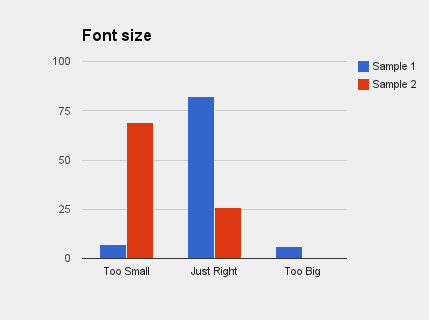
\includegraphics[height=60mm,width=100mm]{fonts.png}
\caption{chart of first year font size preference}
\label{fig:label}
\end{figure}
As this questionnaire was performed in one of the big lecture rooms (Huxley room 311) the preferred sample was the one with the bigger font size (see figure~\ref{fig:label}).
However, as the smaller font size sample is perfectly readable on the lab machines we are considering to release our debugger in two modes: `normal mode' (to be used on the lab machines - font size 16) and  `lecturer mode' (to be used by lecturers when teaching - font size 26).
This was not part of our initial plan but after consulting with our project supervisor, we amended our list of extensions adding a `lecturer mode' to it.

\subsection{System Design}
\todo{Not sure what we should talk about here}
\section{Implementation}

\subsection{Overview}
Deeva is written as a web application in three parts: frontend-server-backend.
A Javascript frontend using Angular, Codemirror and D3, a Java backend using the jdi library to run and control the inferior program and finally a Python web server using Flask and py4j to tie the two together.

\subsection{Deciding on a Web Front End}
From the beginning of this project we knew that the tool would need a graphical interface and so, we were faced with a difficult decision.
The obvious approach was a classic monolithic Java application\footnote{Java being the natural choice since it was the target language}, however, this had some disadvantages.

Firstly, we all have limited experience with desktop GUI programs which meant that it would have been more difficult for us to achieve our projects' goal state.
Secondly, we knew we would need a lot of custom code for drawing the visual program state.
Rendering that in Java would have been a slow and painful process that could have distracted us from actually implementing our core functionalities.
Another reason for not choosing a desktop app is that we found Java UI to be visually unappealing for users.
Finally, Java desktop applications can easily turn to unmanagable-sized projects mainly due to the fact that basic but powerful functionalities that \texttt{Html} offer would need to be reimplemented.
Also, the tool would end up being a complicated application that does not appeal to users which would defeat Tristan's goal of increasing the usage of debuggers among first years.

Therefore, after taking all the above mentioned arguments in consideration we decided to build Deeva as a web application as we have considerably more experience in web developpment that in desktop app developpment.
Also, having examined Python Tutor we knew that the custom UI we wanted would be easy to do in a web front end by using well tested and well documented libraries.
Finally, writing the project as a ``local web service" promotes a clear boundary between interface and backend allowing us to be more efficient at work on the project.
People can work on front and back end simultaneously and allows for either of the components to be easily swapped out.
Also, the decoupling between the frontend and backend component became important when mid way through the project we realised that the lecture room projectors have a low resolution that do not allow for the code and the graphical visual to fit on the same screen.
The solution to this problem became very simple as it only requires to build a customed view for the projectors and connect it to the backend without any additional modifications.

\subsection{Technology Choice}
Deeva uses a range of technologies, some of which were new to us and some which were already familiar.

\subsubsection{Front End}
Effectively all web code ends up being executed in Javascript and although there are many tools which compile to Javascript (CoffeeScript, Dart, TypeScript and many many more) we opted to stick to JavaScript. 
This was mainly due to the fact that all of us had some experience with JavaScript but very little exposure to any of the above mentioned tools.

We decided to use a frontend framework having experienced how messy it was attempting to do without in a second year group project.
Felix had used Angular before and Hector had a some experience with Ember (two Javascript frameworks).
Angular is less opinionated than Ember which fitted better with our slightly unusual project (not to mention Felix's greater experience) so we used Angular.

Our UI includes elements that have fundamentaly differnt purposes.
The code pane where we display code needs to mimic the programming style we are used to and also has to support debugging actions (for example setting breakpoints). 
The state pane where we graphically represent the stack and heap state has to be visually appeling and offer consistent behaviour.
Hand coding these components would have been time consuming and error prone and so, we decided to use and configure existing components in an effort of minimising the NIH Syndrome \cite{NIH}.

For the code pane we used CodeMirror\cite{CodeMirror} as it is a versatile text editor for the browser that is specialised in editing code. 
Also, it has an active community and well-documented API.

For the state pane which shows the graphical representation of the program state we are using D3\cite{D3} as it provides a very easy and powerful way of manipulating data using HTML, SVG and CSS. 
Similarly to CodeMirror, D3 has an active community and a multitude of use cases.

We used Bootstrap\cite{Bootstrap} frontend framework as it provides a fast and easy way to web developpment.
It is generally a popular choice in web developpment as it has multiple extentions and components and it was the natural choice as all of us had previous experience with it.

For the communication architecture between the frontend and the server there are many options but the most common are SOAP/XML and REST/JSON.
We chose to use JOSN and REST partly because it is the one that we have encountered most from the above mentioned options. 
Also, it is simpler than SOAP/XML and is now the de facto standard for new web applications.

\subsubsection{Middleware}
The Middleware is what connects the two seemingly different paradigms and
environments together.  This is where we also map user requests on to the
debugger, and manipulate and convert the data received back from the debugger in
a format that the client expects.  As is recommended, we try not to reinvent the
wheel, especially since it would make us diverge from the main focus of our
project.  Ideally we were looking for a web framework that would sit atop of a
web server, so we could focus more on the debugger rather than how to implement
communication between the server, client and the debugger class (which in turn
is connected to the inferior JVM).

Initially we thought it would be best to use a framework that was implemented on
top of the JVM because then it would mean we could call our debugger code
directly.  Some of the JVM-based frameworks we could have used were:
\begin{itemize}
  \item Play Framework (either in Java or Scala)
  \item Spring Framework
  \item Grails
\end{itemize}

However there was a steep learning curve, and none of us had any prior
experience, which would have meant we would spending less time developing the
debugger, and more trying to figure out how to write a server in one of the
aforementioned frameworks.  This disadvantange, we felt, significantly
outweighed the advantage of being able to natively call our debugger.

For this we resorted to using Flask, a lightweight micro web framework written
in Python, that the majority of us had used and had prior experience with.  It
allows us to get up to speed surprisingly quickly, due to the well designed
nature of the framework and also the language features of Python.  This then
meant we need to find a way of getting the Python VM and the Java VM to
communicate.  Yet again we didn't have time to reinvent the wheel, so we
researched some possible options:
\begin{description}
  \item[Pyjnius]\hfill\\
    Pyjnius is a library which provides methods and protocols for communicating
    between the JVM and the Python VM.  We initially chose Pyjnius, which seemed
    to have an active community and documentation that seemed to be up to
    date. However we quickly realised that there were gaping holes in the
    documentation, and there were many problems.

    Some of these problems included that it wasn't cross-platform friendly, it
    would work on certain platforms, and with a lot of work only sometimes on
    another platform e.g. Mac OS X platform. It also required some C libraries
    that may or may not have needed to be compiled, and the library would have
    to be compiled on every platform it was run, and it is not always guaranteed
    that a C compiler would be present by default e.g. Windows platform
    (although we don't aim to support Windows currently) and also the Mac OS X
    operating systems.

    Another problem we faced with this library was that it more time consuming
    to build, and our tests that the continuous integration server was doing
    took around 15 mins (most of which was spent fetching and getting modules,
    and also building them (especially the compulsory C library that
    \texttt{pyjnius} required).
  \item[JPype]\hfill\\
    JPype is also another library which defines some protocol for which to send
    and receive commands from both the Java and Python virtual machines.

    We briefly considered this option, but the community and the development
    seemed to be inactive, and it didn't seem to pick up a lot of traction in
    the community, meaning if we got a bug, or were unaware how things were to
    be, we would have to investigate ourselves and provide a fix ourselves.

    The documentation also seemed to be unhelpful and very outdated, so we had
    to pass up this option.
  \item[Jython]\hfill\\
    Jython isn't necessarily a framework per-se but an implementation of Python
    on the Java Virtual Machine, meaning it could natively call functions of
    languages that are based on the JVM i.e. Java, Scala etc. This seemed like a
    better alternative than the other JVM based frameworks, as it also had all
    the popular language features and expressiveness of the Python language.

    However appealing this solution was, it had significant drawbacks. We had to
    make sure that all the Python libraries/modules we were planning to use had
    Jython implementations. We couldn't make this guarantee from the start as
    this project was also very exploratory (we didn't know what we needed before
    we needed it).
  \item[\texttt{py4j}]\hfill\\
    Like \texttt{pyjnius} and \texttt{JPype}, \texttt{py4j} also provided
    methods and protocols for communicating between the two VMs. We settled for
    this option because it seemed to be the most stable, and was rather
    intuitive. The developer behind it seemed to be quite active, and a lot of
    bug fixes had been present.

    We did have a few issues, which were in fact bugs, and in the end we cloned
    and forked the repository and made the changes ourselves and when building
    Deeva, we pull from our fork.

    However we've been largely impressed and comfortable with this library and
    would thoroughly recommend it if using Python is a must.
\end{description}

\textbf{Client Implementation}

Aside from the bridging libraries and the web server frameworks, there was more
to the Middleware that wasn't necessarily an integral part of the Java Debugger,
hence may nont be included in the back-end section. This is because we could
swap it out and use a different client, due to the implementation agnostic
approach we took in designing our debugger. This is just one way of implementing
a client to our class, if we were to use Java UI we could still interact with
our Debugger class without any changes to it.

We previously discussed that low resolution was a problem, especially for where
it would be mainly used, in a teaching setting (namely Huxley 308/311) where the
projectors have very low resolution, and even if they had higher resolution they
would not be visible from the back. This forced us to rethink our design, and
was also another reason for why we moved away from the initial semaphore design
we were using. If we were able to have two separate views running, one showing
the main interface (code and state) and another view showing the stack and heap,
then this problem of the low resolution could be alleviated.

\textbf{\emph{Blinker, Event Dispatching, Event Stream, Server-Sent Events}}

To achieve this we needed a way for multiple clients (be it objects/threads
etc.) to simultaneously get data from the debugger. This couldn't happen with
the semaphore approach, since we could only deal with one request at a time, and
also the requests are independent of each other and are unaware of each other.

Enter \texttt{blinker} ``Blinker provides fast \& simple object-to-object and
broadcast signaling for Python objects.'' \cite{blinker}. This allows us to
define signals/events, and also subscribers that would subscribe to these
events, similar to the Publish-Subscribe model. This ties in with the Event
Dispatcher that was previously aforementioned, when the inferior JVM emits an
event, which then gets handled by our Debugger, which then calls methods defined
in the Dispatcher passed whilst being created. Our implementation of the
\texttt{DeevaEventDispatcher} then sends a signal using \texttt{blinker} to all
those who are listening/subscribed.

The idea is that due to the asynchronous nature of the debugger, each view gets
data pushed to it via some event stream, containing the relevant bits of data as
and when it happens. Each view can get this data pushed to it by subscribing to
the relevant signals that the EventDispatcher defined, e.g. a stack/heap view
would only subscribe to events pertaining to the stack/heap and also control
events that determine the state of the debugger.

So currently we have a way of getting a stream of data that the debugger is
outputting, and we can have multiple listeners, however, how can we push this to
the client browser? There were two possible options that we considered with
regards to server-to-client push in real time: Websockets and Server-Sent
Events.

We have had previous experience with Websockets, which was useful for providing
real time functionality in both directions, however it required a complicated
setup, and seemed overkill. Also client-to-server needn't happen in real time
and could be handled with just simple \texttt{POST} requests.

This is where Server-Sent Events (SSE) come into play, this technology keeps the
connection between the browser and the server open so that the server can just
continually write more and more data in one go without ever closing the
connection, achieving some sort of pipe functionality with streaming. We also
define events that the browser would listen for, and on the front-end
javascript, we define event handlers for such data.

So overall, the client would open a \texttt{eventstream} connection, which in
turn would create a new subscriber to all the relevant signals as previously
mentioned, so that when the inferior JVM emitted events which in turn cased the
debugger to emit events (via the Event Dispatcher), which in turn sends signals
using \texttt{blinker}, and the data would be pushed all the way from the JVM to
the client and be processed and displayed as need be.



\todo[inline]{EventDispatcher Implementation - I/O}
\todo[inline]{SSE}
\todo[inline]{Blinker/Stack Heap view}
\todo[inline]{Diagram showing the model - maybe it should go in the design bit}
\todo[inline]{Data processing into a format the client was expecting}
\todo[inline]{Loading the files}
\todo[inline]{Starting the debugger,}
\todo[inline]{User experience, files out of date}

\subsubsection{Back End}
\textbf{Java Virtual Machine Tools Interface (JVM TI) and the Java Debug Interface (JDI)}

The Java specification provides an interface that all the different JVM implementations must conform to (of course, some features may not be supported in some Virtual Machines (VMs) for which the specification provides for).
The Java Virtual Machine Tools Interface (JVM TI) \cite{jvmti} allows a program to inspect the state and control the execution of applications running in a JVM.
This API is written in C/C++ and is quite low level (in fact it is the lowest in the Debugger Architecture).
Java provides another interface written in Java, the Java Debug Interface (JDI), which wraps JVM TI calls in Java so that a Java program can manipulate the state of another JVM.
This is useful as it simplifies our process, as we don't have to worry about wrapping Java to call C functions and vice versa, and also get the correct semantics, (the JDI library is quite huge, and implementing it ourselves is another project in itself).

With this in mind, we first thought that implementation would be quite simple, however we misunderstood the model of how the JVM works together with JDI.
The inferior JVM (the virtual machine hosting the program being debugged) has to run in a separate virtual machine, because if the debugger and the debuggee run in the same virtual machine, a catastrophic bug in the program debugged can crash the debugger, rendering it useless.
The inferior JVM probably has no knowledge that it is being ``debugged'', and having them in the same process/JVM most probably increases the liklihood of Heisenbugs \cite{heisenbug}.

A JVM can emit events when certain things happen e.g. when a thread is suspended, when the VM has been initialised or killed, when a breakpoint has been reached, when a method has been entered/exited, and when a single step has occurred (either step into, step over, step return).
What a debugger would do, would define an Event Handler, which listens and processes the events that are emitted.
However if a JVM were to output every possible event, it would cripple execution time (plus the JDI can be used for instrumentation i.e. generate a stream of trace where the original source can't be modified).
The solution to this is that we submit requests for events we would like to handle, and define methods that would be called should we see an event.

\textbf{Deeva - Java Debugger Implementation}\\
Our debugger is not a fully fledged one, however we believe it suffices for the scope of our project.
It consists of mainly three parts, an Event Loop, Event Handler, and a general class that can make requests to the JVM.

\textbf{\emph{Event Loop \& Event Handler}}\\
The Event Loop runs in a separate thread, and it is connected to the inferior VM, listening for any requests that were submitted.
When it receives an event, it will then call a suitable handler to handle that event.
We only define handlers for events that we wish to handle, i.e. events that are in the scope of our project.
The information we wished to capture and return back to our client listeners are not always contained within a single class within the JDI, and can be spread everywhere.

To ameliorate this, we made some simple Plain Old Java Objects (POJO) to contain the state we wished to capture and communicate to clients using our library.
Initially we were using HashMaps to contain state, because that would work well with Python's dictionary types; however there were many caveats due to way that \texttt{py4j} mapped Java collection types and Python's collection types and serialisation became a big issue and if we had continued down this path we would have classes that had members that were unrelated.

Encapsulating the state that we wanted in POJOs meant that we could run serialisers, like \texttt{gson} (which serialises a Java Object into the JSON format) and we could deserialise the JSON on the Python side, into the Python Dictionary without any complaints.
This method is more desirable because JSON is a public standard, so should anyone want to use our debugger library (in a different environment other than Python or Java), they would have a standard way of getting data out of our library.

\todo[inline]{Talk about state data generation, object references/primitive types}

\textbf{\emph{General Request Class and Event Dispatching}}\\
This is class that clients (and in our case the Python VM via py4j) interacts with.
We can make our requests which then forwards the request onto the inferior JVM.

Due to the asynchronous nature of the JVM and it's events (the reason why we first misunderstood the model), we needed another way of receiving and processing the events, cue our Event Handler as aforementioned.
However that was only one step of the process, we also needed to asynchronously communicate the data from the events (that we had subscribed to).

Initially we had used a semaphore, so that requests didn't complete until an event that would suspend the JVM would come and release the semaphore, thus sending the state back with the initial request.
This created problems because of threaded nature of our web server, and the threaded nature of py4j and we were often getting deadlock, or being in inconsistent states (as the web interface wouldn't respond as the request was blocked or a deadlock etc).
It also meant that we couldn't define a new view of the state of the debugger, hence our Python web server would be tightly coupled to the inner workings of the debugger (i.e. requests blocking whilst blocking on a semaphore, which could only be released by a suspending event).

We addressed this by defining an interface \texttt{`DeevaEventDispatcher'}, where clients would implement this interface and pass it into the constructor for our library, i.e. callbacks or handlers that get called when we're handling JDI events, e.g. should we receive a Breakpoint event, we then call \texttt{`suspended\_event()'} and pass along the state object.
The concrete implementation of this on the client side would define the behaviour or what should happen should our debugger report that the JVM has suspended.
How we implemented this for our client side is mentioned below in \emph{Middleware}.

\textbf{\emph{Input/Output (I/O)}}\\
Most first years are unlikely to have been introduced to Java UI and that also requires an understanding of how Java works as a whole.
This makes input and output via \texttt{stdin} and \texttt{stdout/stderr} respectively paramount, as they would be writing to and reading from the command line.
Implementing support was split into two parts: input and output.

How we handled output was that we had a separate thread running for each type of output (\texttt{stdout \& stderr}). We started this thread when the inferior JVM was started and we would redirect the outputs of the inferior JVM to their respective threads.
The thread would then make a call to the event dispatcher, signalling that output had occurred, and we would send the output along with it.

How we handled input was different, and we also had to take into account the thread running the I/O request could block waiting for input.
Basically there is a \texttt{BlockingQueue} on the Java side in our debugger, that contains the data from a ``command line''.
There was a separate thread running that would pull data from this queue, and then feed it into the \texttt{OutputStream} that is connected to the \texttt{InputStream} (i.e. \texttt{Standard.in}) of the inferior JVM process.

However we still had to deal with the problem that occurred when the thread running the main function would block waiting for input.
Taking into consideration our development stack, we had to provide a way of informing the user that we were awaiting data, otherwise it would look like the site (client view of debugged program) had frozen.

We mitigated this problem by adding a hook into the debuggee JVM.
This hook found the \texttt{System.in} object, and we made a \texttt{MethodEntryRequest} whenever \texttt{read()} was called (which it is called implicitly by \texttt{InputStreamReader}s, \texttt{Scanner}s etc.)
We had to use this method of ``monkey-patching'' since for \texttt{System.in}, \texttt{read()} is a native call which is also blocking, and as a result the state of the thread (in Java) performing the call would still be \texttt{RUNNING} as if it isn't blocked (a caveat of the JVM).

When the inferior JVM starts to read from input, the JVM would suspend and emit an event.
Whilst the JVM is suspended, we can also invoke methods.
The \texttt{InputStream} class has a method called \texttt{available()} which as described by the Java docs: ``Returns an estimate of the number of bytes that can be read (or skipped over) from this input stream without blocking by the next invocation of a method for this input stream.'' \cite{java_available}.
It is usually not advised to use this value as part of a decision process, however we were in complete control of the inferior JVMs \texttt{stdin}, as it is backed by a Queue.

We couldn't have put this logic in the Thread that was ``redirecting'' input, because it would keep notifying the user especially when the Queue was empty i.e. no data was entered in by the client.
This way allows us to inform the user that we are ``requesting'' data (even though in the command line this rarely happens).
It also allows the user experience to be more intuitive, especially considering our target audience and our development stack (i.e. web application).

How we handled I/O when it got to the client is mentioned below in \emph{Middleware}.

\todo[inline]{Insert diagram of how I/O redirection worked}

\textbf{\emph{Sourcepath/Classpath resolution}}\\
Since our debugger should be able to be run from anywhere, and also we can't assume that compiled sources would be in the same directory as the source files themselves, we tried to do some form of classpath/sourcepath resolution.

The user would specify a classpath as usual, but also they had to specify a sourcepath, so we could find the corresponding sources for the classes that had been loaded.
By default, to conform with Java's semantics, if they don't specify a classpath/sourcepath, we assume that it is just the current directory.

To find all the classes that could potentially be of interest (N.B. we couldn't find a way that would  determine exactly what classes we would need before hand, see \emph{Classloading} below.) we traversed the directories listed in the classpath, looking for class files.
Should we find a class file, we would append the directory structure relative to one of the directories in the classpath, so we could get the fully qualified class name (e.g. \texttt{java.lang.String} rather than just \texttt{String}).
We would then keep a track of the absolute path of this class in map to be used later.

To find all the sources, instead of adding any source file, we would only add sources that had a corresponding class that had been detected by the algorithm described above.

Clients could then query this set of data, and load the source files for classes they were interested in (lazily).

\textbf{\emph{Error Handling}}\\
The JVM is a complicated piece of software, we can also think of it as a software processor (since it also has it own instruction set).
So it goes without saying that JVM errors are bound to occur.
On top of that there could be errors as part of the debugging process.

So it is imperative that we handle these errors in a nice way, and communicate that to the client.
In our debugger, we can catch those errors via Exceptions, but that is native to our debugger, it still needs to be communicated to the client.
We can make use of our event dispatcher as aforementioned (\texttt{DeevaEventDispatcher}), which we can pass a nice description of the error, and it can be later handled by the client.

A few examples of errors that we handle are:
\begin{description}
  \item[AbsentInformationException]\hfill\\
    This exception is raised when we try to query the JVM for knowledge that would only be there should the class file we're interested contains it, but isn't i.e. the class file was not compiled with debug symbols.

    The main piece of information that we're interested in is the mapping of Java bytecode to line numbers in the source code.
    Without it we're unable to invoke a lot of methods, as we don't have the required information, also it doesn't make sense either, and would just turn our program into a glorified program runner.
    How we handle this is to send a message through the \texttt{DeevaEventDispatcher} that we have an error.

  \item[VMDisconnectedException]\hfill\\
    This exception is raised when we try to request an operation on the inferior JVM, however the VM in question is no longer accessible.

    This could happen if the program running in the inferior JVM has finished running, and the user manages to get a request in.
    Like previously mentioned, we send a message through the \texttt{DeevaEventDispatcher} about this error.
\end{description}

\textbf{\emph{General Problems/Caveats}}\\
As with most projects, things don't always go as planned, and we generally run into problems, the main concerns that we ran into were thread safety, (this was particularly important due to our choice of development stack), and also the way that Java did class loading and the implications it had for us.

\emph{Thread Safety}\\
The libraries \texttt{py4j} and \texttt{Flask} are thread-safe, however access to objects in Java are not i.e. the Debugger class that the client will interact with needs to have synchronisation primitives.
This is because every request made by the user in the browser results in a separate thread being created to handle that request.
Any call using \texttt{py4j} also creates a new thread to deal with that request.
Hence $x$ requests from the browser results in $x$ threads trying to access the Debug object, and we must also take into account the Event Handler thread that writes to our Debugger class.

As a result we had to group certain methods together and control access to them using a lock (implicit - Java's synchronisation keyword and the explicit Lock class).
This is to ensure mutual exclusion and that the data is consistent between requests, and also to irradicate race conditions.

This is also why we had to switch from semaphore approach we described earlier, because should something go wrong, threads from Python would get stuck waiting for threads in Java to unblock, but they were blocked by some other thread etc. thus greatly complicating an already complicated thread model.

\emph{Classloading}\\
A problem we encountered was when we were trying to set breakpoint, we were unable to tell beforehand whether a location of a given breakpoint was valid.
By valid we mean that we can't breakpoint on an empty line or something that was not an executable piece of code.
The JDI does support methods for detecting when this happens, however we can't check this until the class has been loaded.
Without any source code processing, the best thing we could do were to save the breakpoints in a map and attempt to set them, should we have a \texttt{ClassNotLoadedException}, we can save that breakpoint to apply later.

This is mainly due to how Java works. It doesn't load all the classes that would be needed at the same time, it lazy loads them (i.e. as when and they are referenced/needed).
Also it is not advised to force class loading, especially as some programs can dynamically modify the classpath at runtime.
Another reason is that Java also supports custom class loaders, so we may not even be able to force load a class, as it has been defined by a custom class loader of which we can't determine how it loads classes before.

Considering the scope of our project, it may have been safe to assume that first year students who require a simple debugger wouldn't necessarily be using custom class loaders.
Trying to process the source ourselves to determine which lines are okay, probably would have meant invoking the compiler, or trying to decompile class files and look at the mapping or something along those lines, which would have added greater complexity to our project which is currently out of scope, (however this would make an interesting extension and add to the user experience).

\section{Evaluation}
\label{sec:evaluation}
We used a number of techniques to evaluate Deeva.
We used some techniques to help us find or fix specific problems and we used others to make sure that we were on the right track building the right things.
\subsection{Usability Testing}

\subsubsection{Hallway Testing}
\begin{figure}[h!]
\centering
\subfigure{%
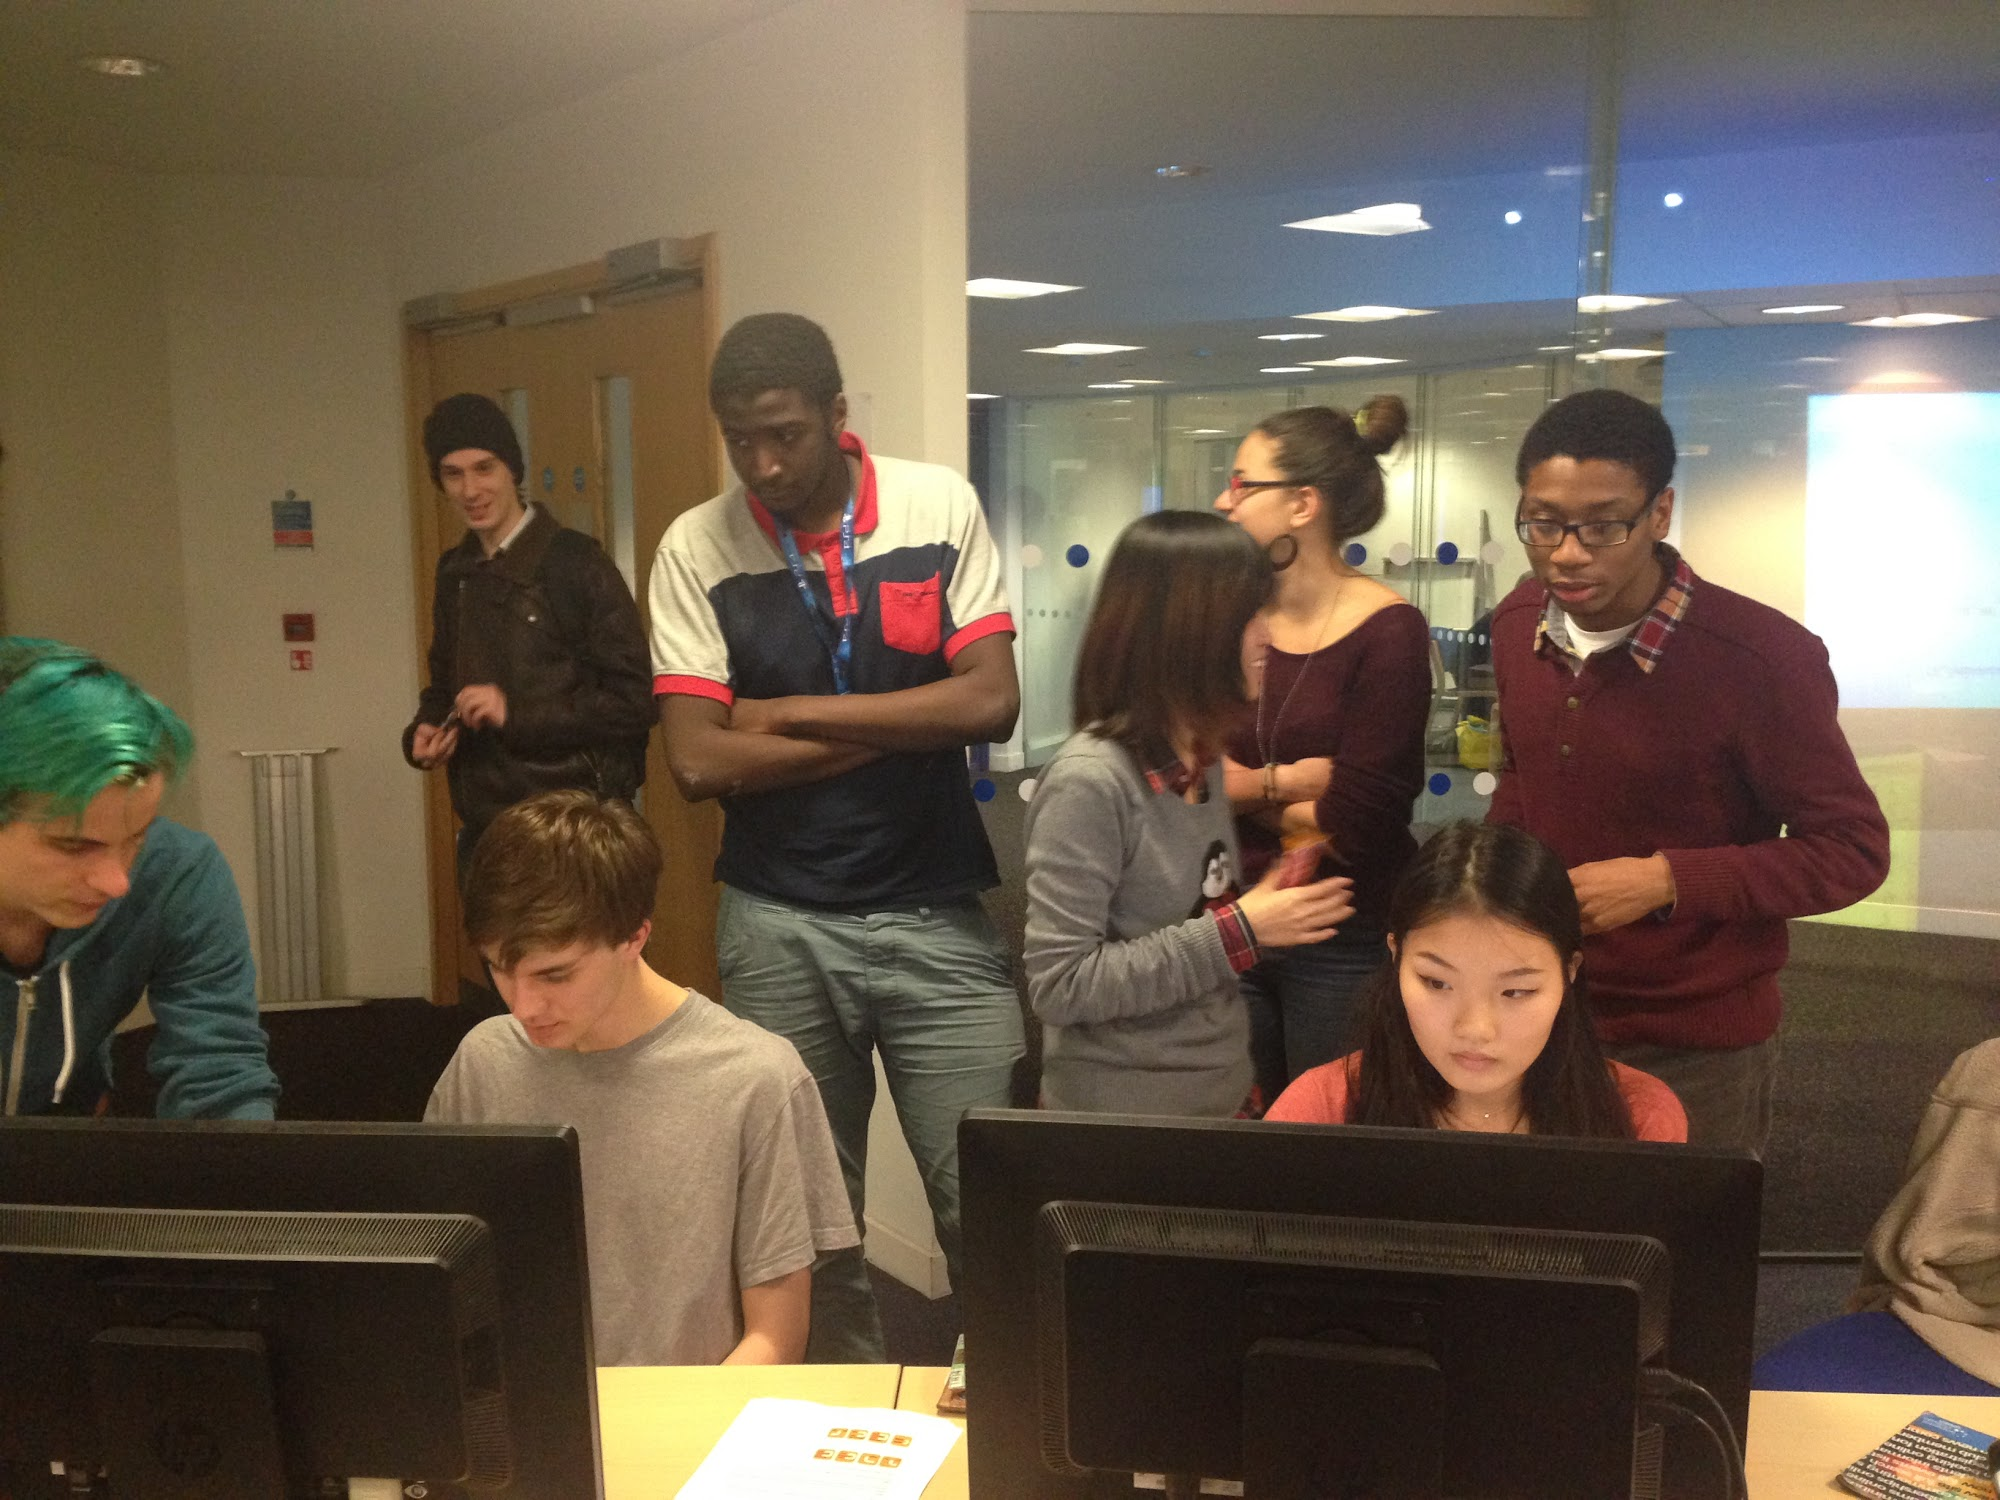
\includegraphics[height=50mm, width=60mm]{hallway1.jpg}}
\quad
\subfigure{%
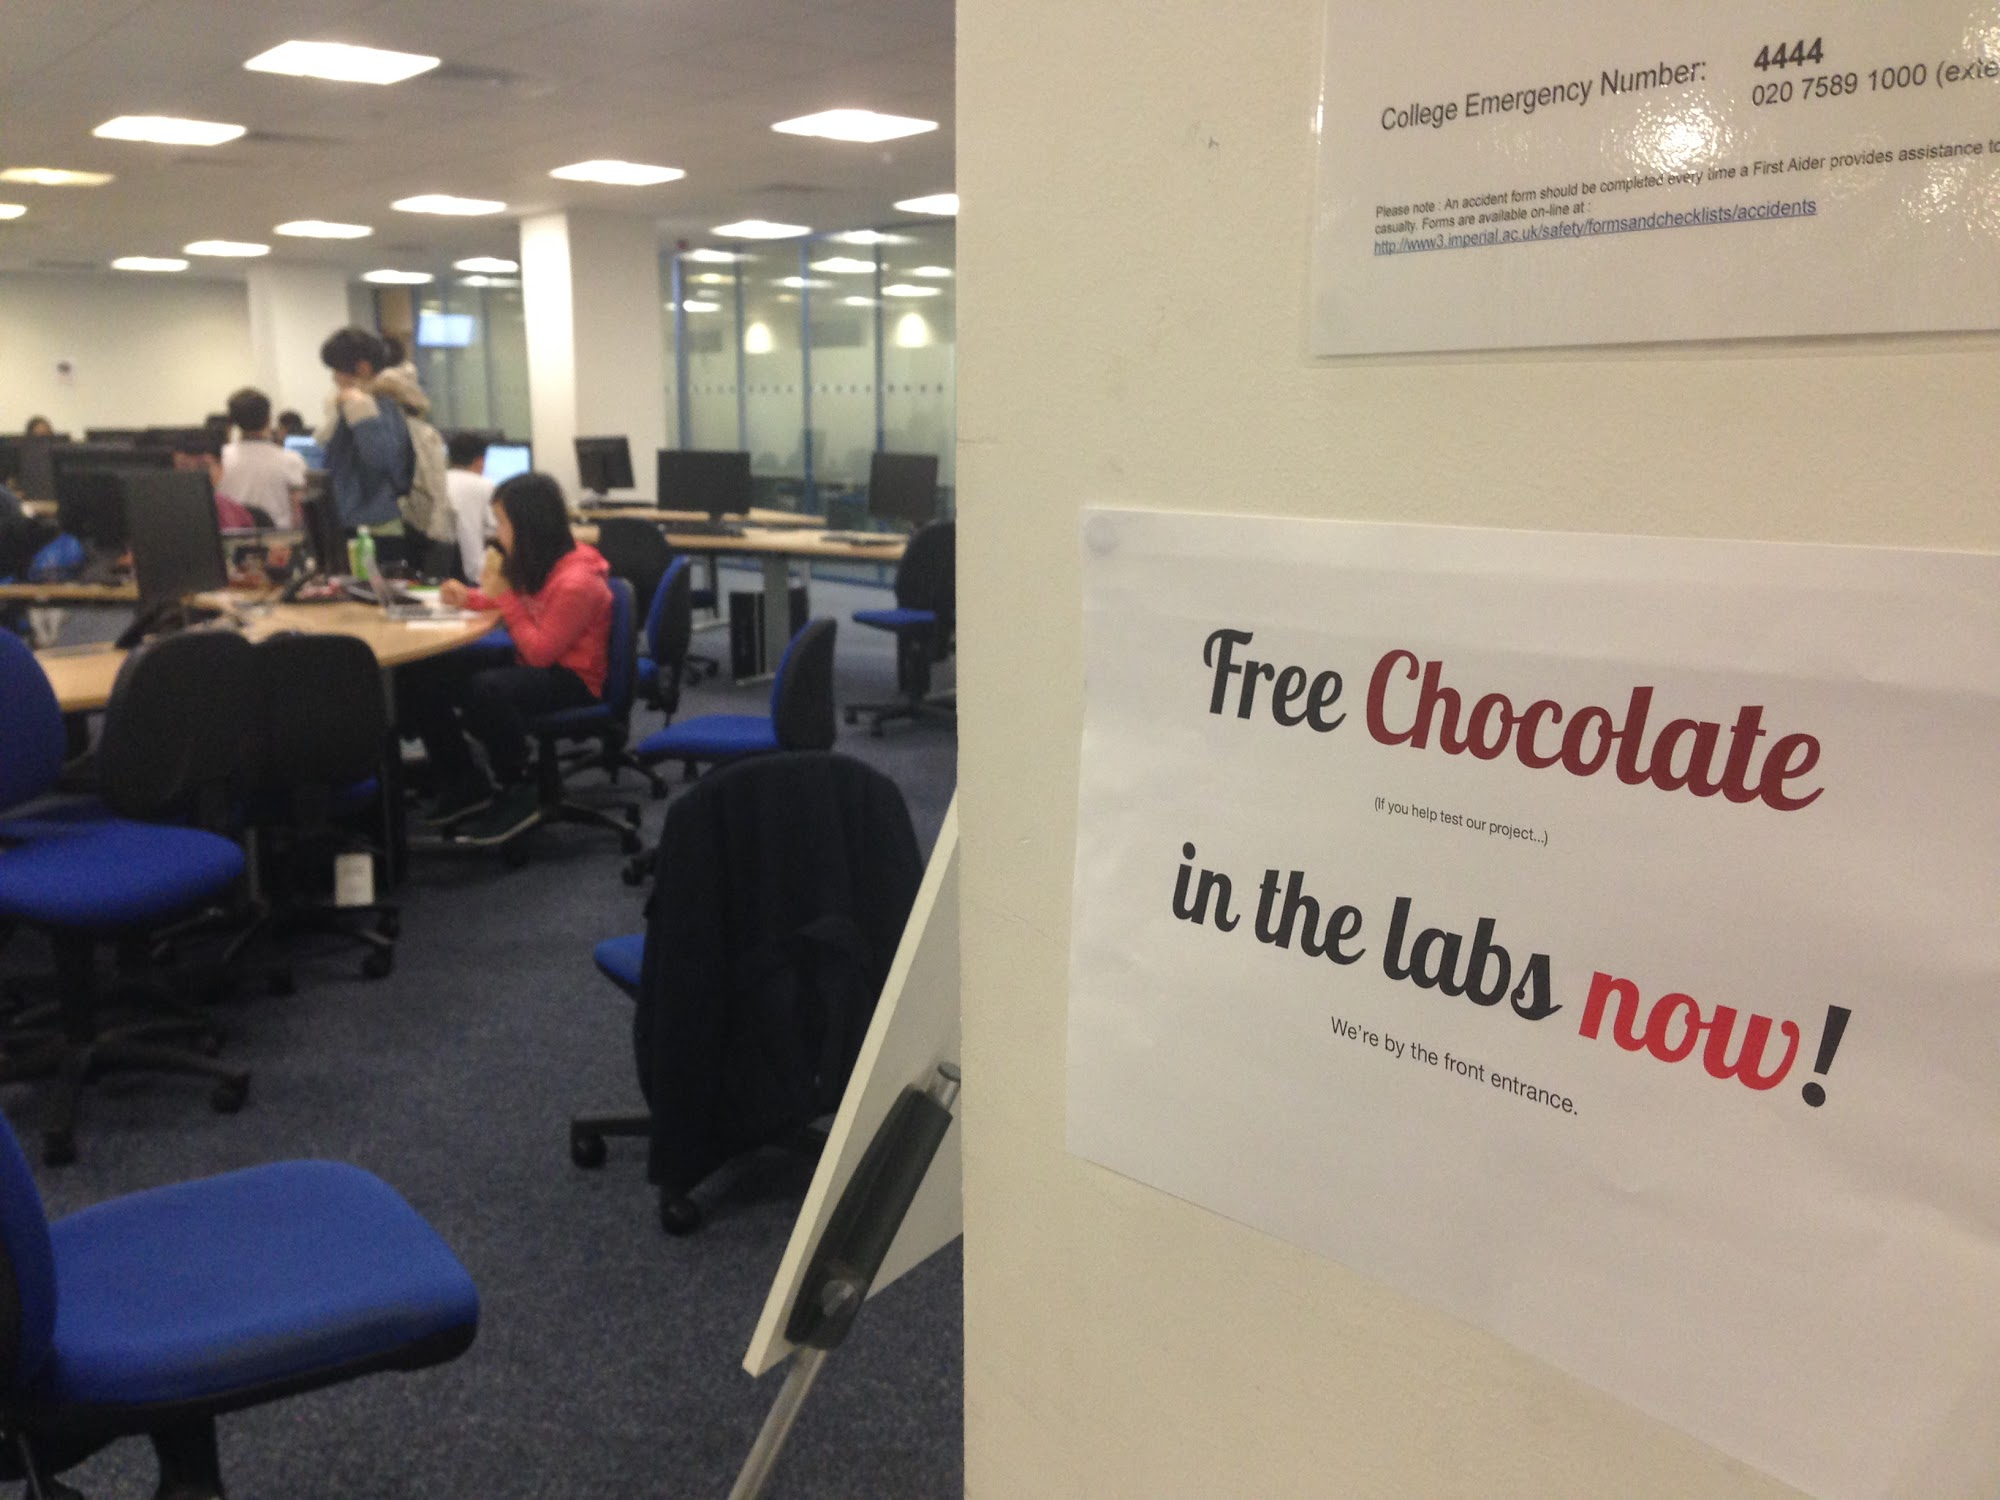
\includegraphics[height=50mm, width=60mm]{hallway2.jpg}}
\caption{The pictures taken during Hallway Testing}
\label{fig:hallway}
\end{figure}

We employed a hallway testing approach when it came to evaluating the usability of our debugger, by getting the first year students (our primary stakeholders) and some second year students to demo our project and tell us their first impressions and what they were expecting (see figure~\ref{fig:hallway}). This was beneficial because as the developers, we are aware of the caveats and may subliminally navigate around them.
Using the feedback from first year students allowed us to identify critical bugs/pitfalls in our usability design.
This was obviously more qualitative however we used some measures (like how many times they had to ask questions) to help quantify things such as how intuitive the interface was or feature complete it was.
On average, the people who participated in the testing asked around 1-3 questions related to basic features like how to run Deeva or how to set a breakpoint.
This was insightful as we are aiming to make Deeva as intuitive as possible so we minimise the need to consult the help menu.
This helped mainly with our first use case which is students using Deeva on the lab machines.

\subsubsection{Quantified testing of colour schemes and font sizes}
We wanted to employ the use of A/B testing to assess how effective certain colour schemes and font sizes would be.
However we had to make a compromise, because the environment and number of users that we could get in one room simultaneously meant that we had to do it in one sitting i.e. we could not force half the users in the room see one colour scheme and the other half see a different colour scheme.
So in the end we just conducted a poll so they could pick which colour scheme and font size they liked the best.
We did this with the help of our project supervisor (who lectures the course in which our debugger will primarily be used).

This is helpful as it allows us to catch possible problems with readability early, which in our case may change the direction in which our solution is architected.
An example of this is that the projectors’ resolution in the lecture room is small, so not all the necessary information can be seen.
Hence, we may need to have a separate mode which shows just the stack and the heap.
The implication of this mode meant we had to change our implementation to be less monolithic.

\subsubsection{Questionnaire}
\begin{figure}[h!]
\centering
\subfigure{%
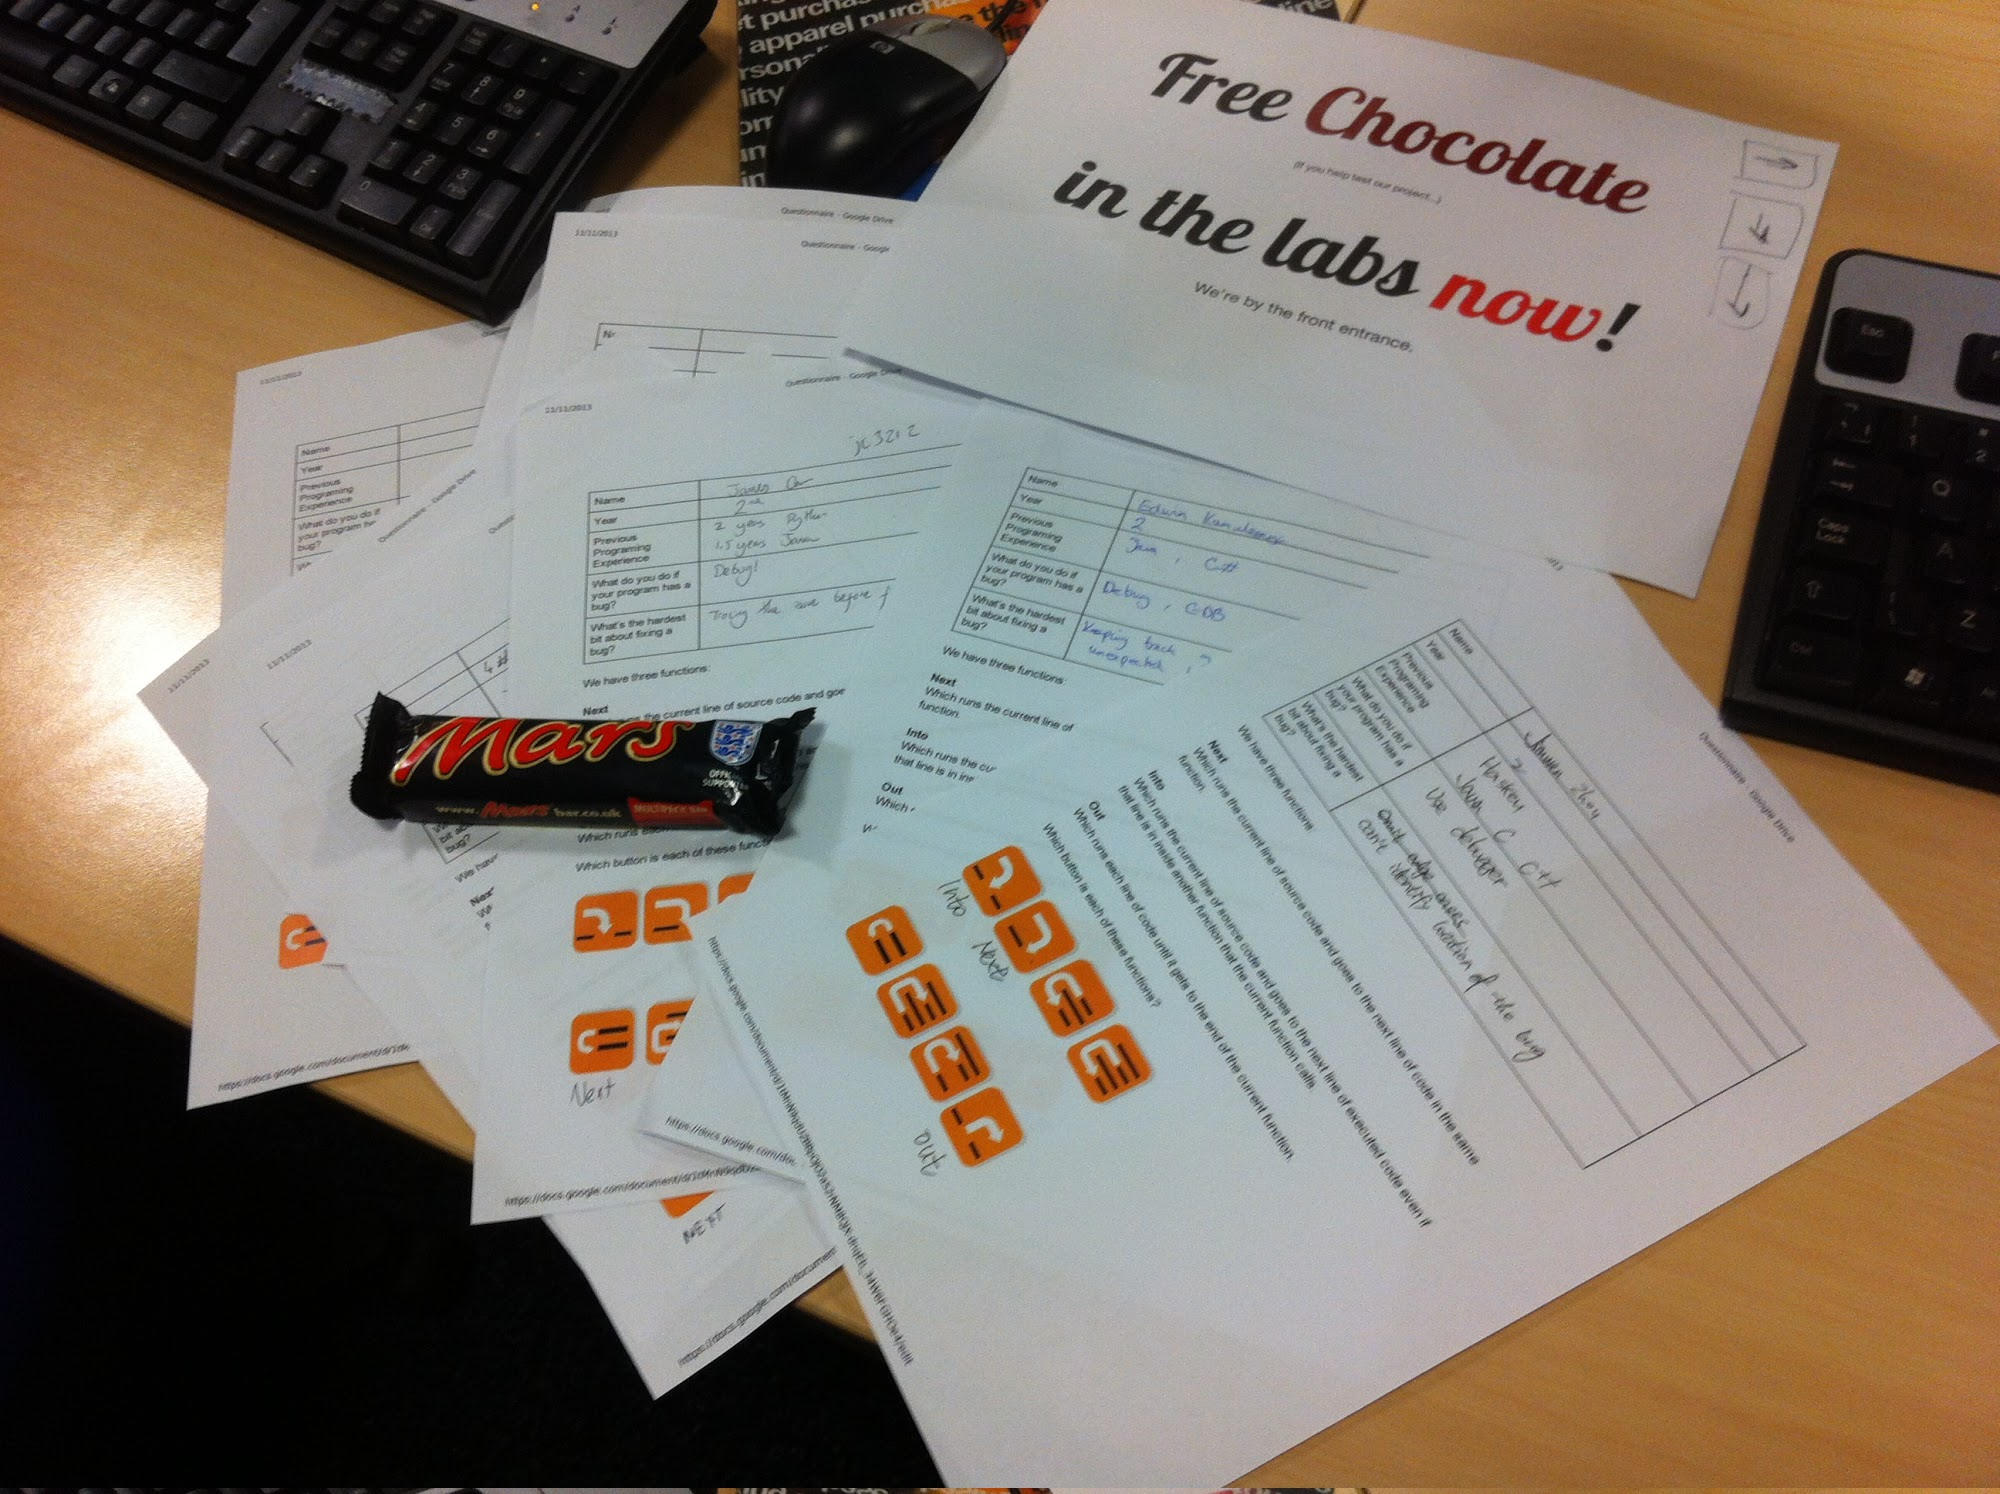
\includegraphics[height=50mm, width=60mm]{questionnair1.jpg}}
\quad
\subfigure{%
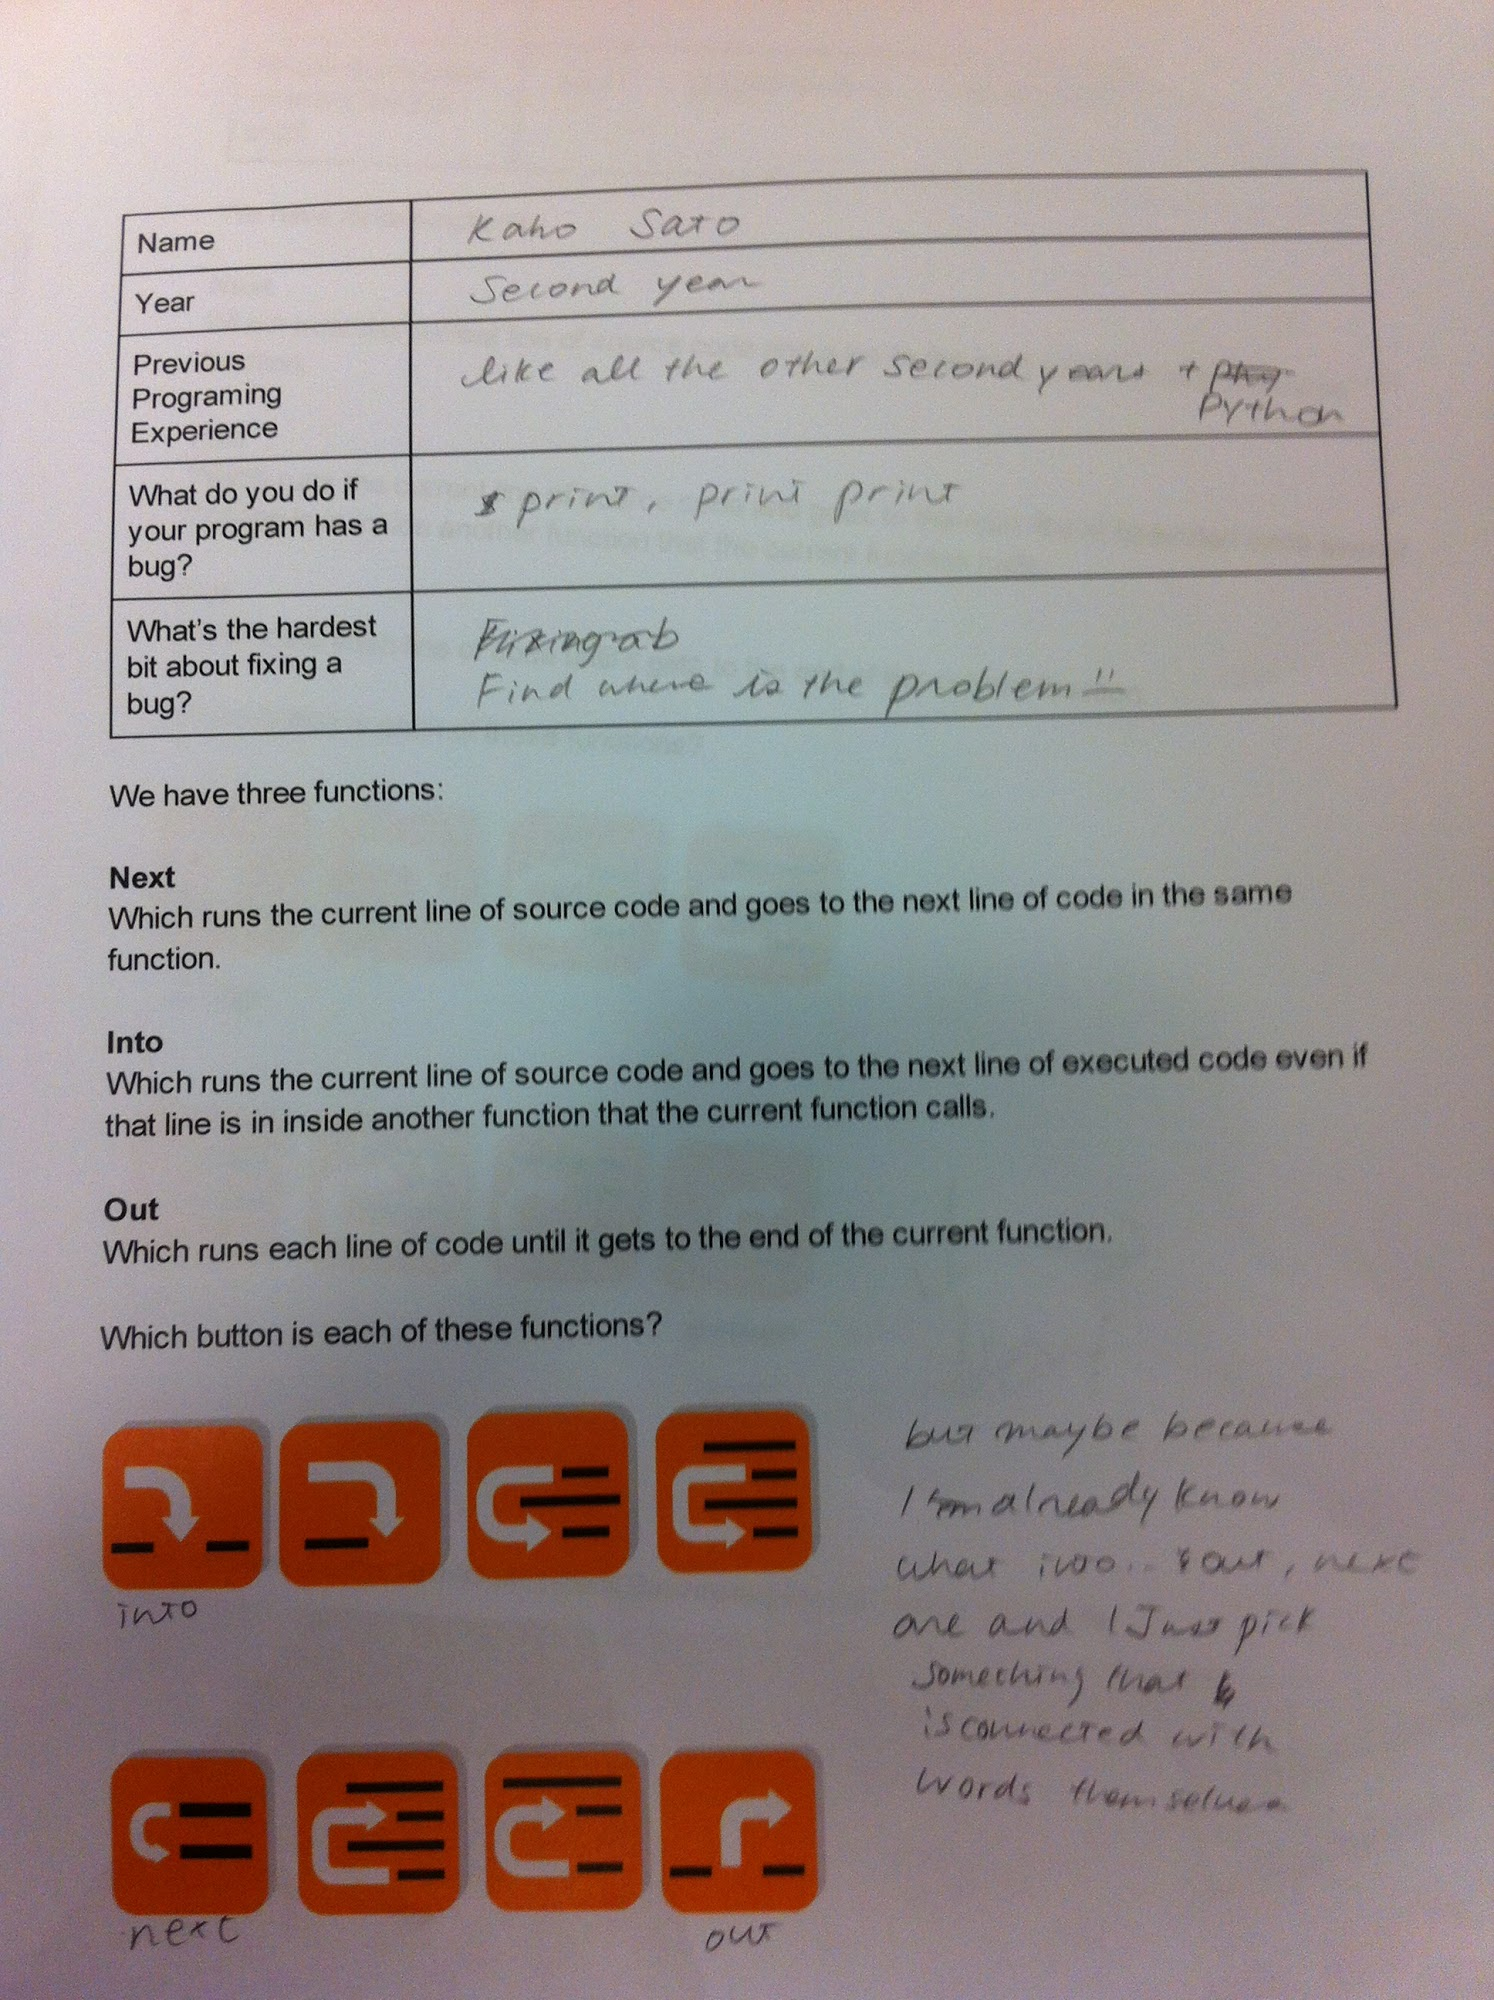
\includegraphics[height=50mm, width=60mm]{questionnair2.jpg}}
\caption{Questionnaire examples}
\end{figure}

After the general interviews we used a questionnaire to get answers to our most important questions.
Specifically we asked which of the several button designs were better and validated our ad-hoc interview conclusions about the debugger.
We considered using something like Amazon Mechanical Turk to get larger numbers of responses which might have been more statistically significant but it seemed silly when we had hundreds of programmers who were our exact target audience sitting next to us.


\subsection{Performance Testing}
We also used a few other metrics, some custom and some off-the-shelf which could be automatically run over the repository to measure specific aspects of Deeva’s performance.

\subsubsection{Time to First Request}

\begin{figure}[h!]
\centering
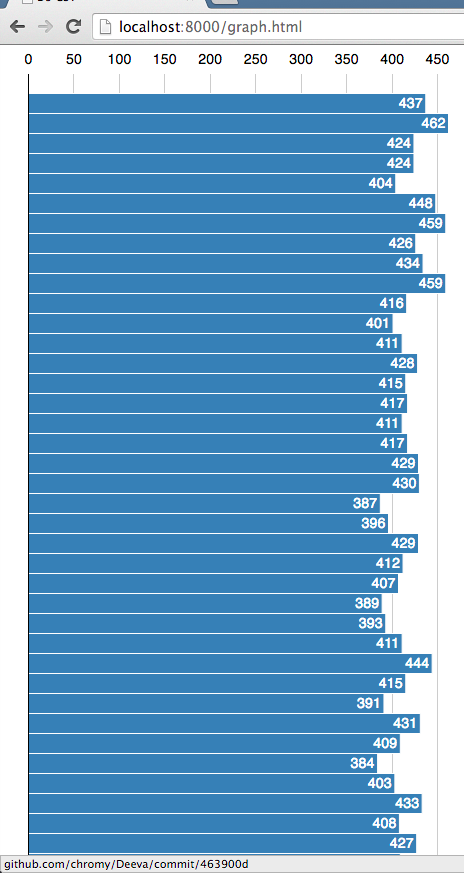
\includegraphics[width=100mm]{timeToFirstRequest.png}
\caption{Custom D3 graph displaying  time to first request}
\label{fig:timeToFirstRequest}
\end{figure}

One of these was the `time-to-first-request'.
This is the time it takes Deeva to get from hitting enter on the command line to being able to accept user input.
This is important because tools that are slow to start are painful to use and hence are used less\footnote{It's not a direct parallel but if we consider websites, page abandonment approaches 50\% as load time reaches about 10 seconds see: \url{http://blog.kissmetrics.com/loading-time/?wide=1}}.
You can only improve what you measure so we wrote a script that iterates over the git history, starts Deeva and measures the time until it is accepting the first request\footnote{We got the idea for doing this from Gary Bernhardt screencast: \url{https://www.destroyallsoftware.com/screencasts/catalog/time-to-first-request}}.
We can then display the results using a custom D3 graph.

From figure~\ref{fig:timeToFirstRequest}, you can see our application takes roughly 450ms to load.

This graph allowed us to see when a commit increased the time-to-first-request, by clicking on the offending bar we could go to the relevant commit on Github and workout what caused the regression.

Happily this turned out not to be such a big issue on this project as the time-to-first-request quickly stabilised and did not increase dramatically.

\section{Project Management}
This project has probably been the largest and the most intricated we ever had to build.
Along with the nature of the project, it combined three major milestones that we never had to face before (at least in combination): we are not sure what are we building, we want to make sure we deliver the software on time but we do not know how long it will take and we want to make sure the software we write is correct and useful but it is hard to define `correct' or `useful' in this context.

\subsection{Agile Programming}

Our software devlopment process is based on Agile programming methods because we found the approach suitable for our goals for the project. 
On top of helping solving the above mentioned challenges, Agile programming has sustainable methods for dealing with large, volatile projects.

Firstly, it is based on iterative development, promoting tight cycles. 
Because this was a large project for which we were not sure how many features we can fit in the allocated time constrains, using one week development cycles helped us to keep track of the team's general speed and setbacks. 
For examlple, we could see in which weeks we were busy doing other courseworks and the number of implemented features in that cycle was low. 
We than could compensate by redesigning our goals for the next cycle. 
This introduces another key feature of Agile programming: flexible response to change.

One of our main challanges was the uncertainty regarding the end result of the project. 
Hence, we required a programming style that allowed for rapid response to change as our initial plan changed during the project execution.

Finally, incremental feature development allowed us to have a basic tool working soon after the project assignment which meant we started receiving feedback from the early stages of Deeva. 

\subsection{Team Management}

To ensure effective development of the product, weekly supervisor meetings were scheduled.
In these meetings, quality assurance was the main aim, making sure we were on the right track with our development, delivering correct features.
This avoided unnecessary misunderstandings and extra time spent on creating unneeded features for the product.

Further to the supervisor meetings, weekly group meetings ensured that all group members are in sync about the progress and direction of the project.
During these meetings, the information gathered from the supervisor meetings would be recapped and the targets for the upcoming week would be set.
Thus, tasks could be divided among group members, with everyone knowing what their colleagues are working on in this week, making group and individual efforts significantly more effective.
\begin{figure}[h!]
\centering
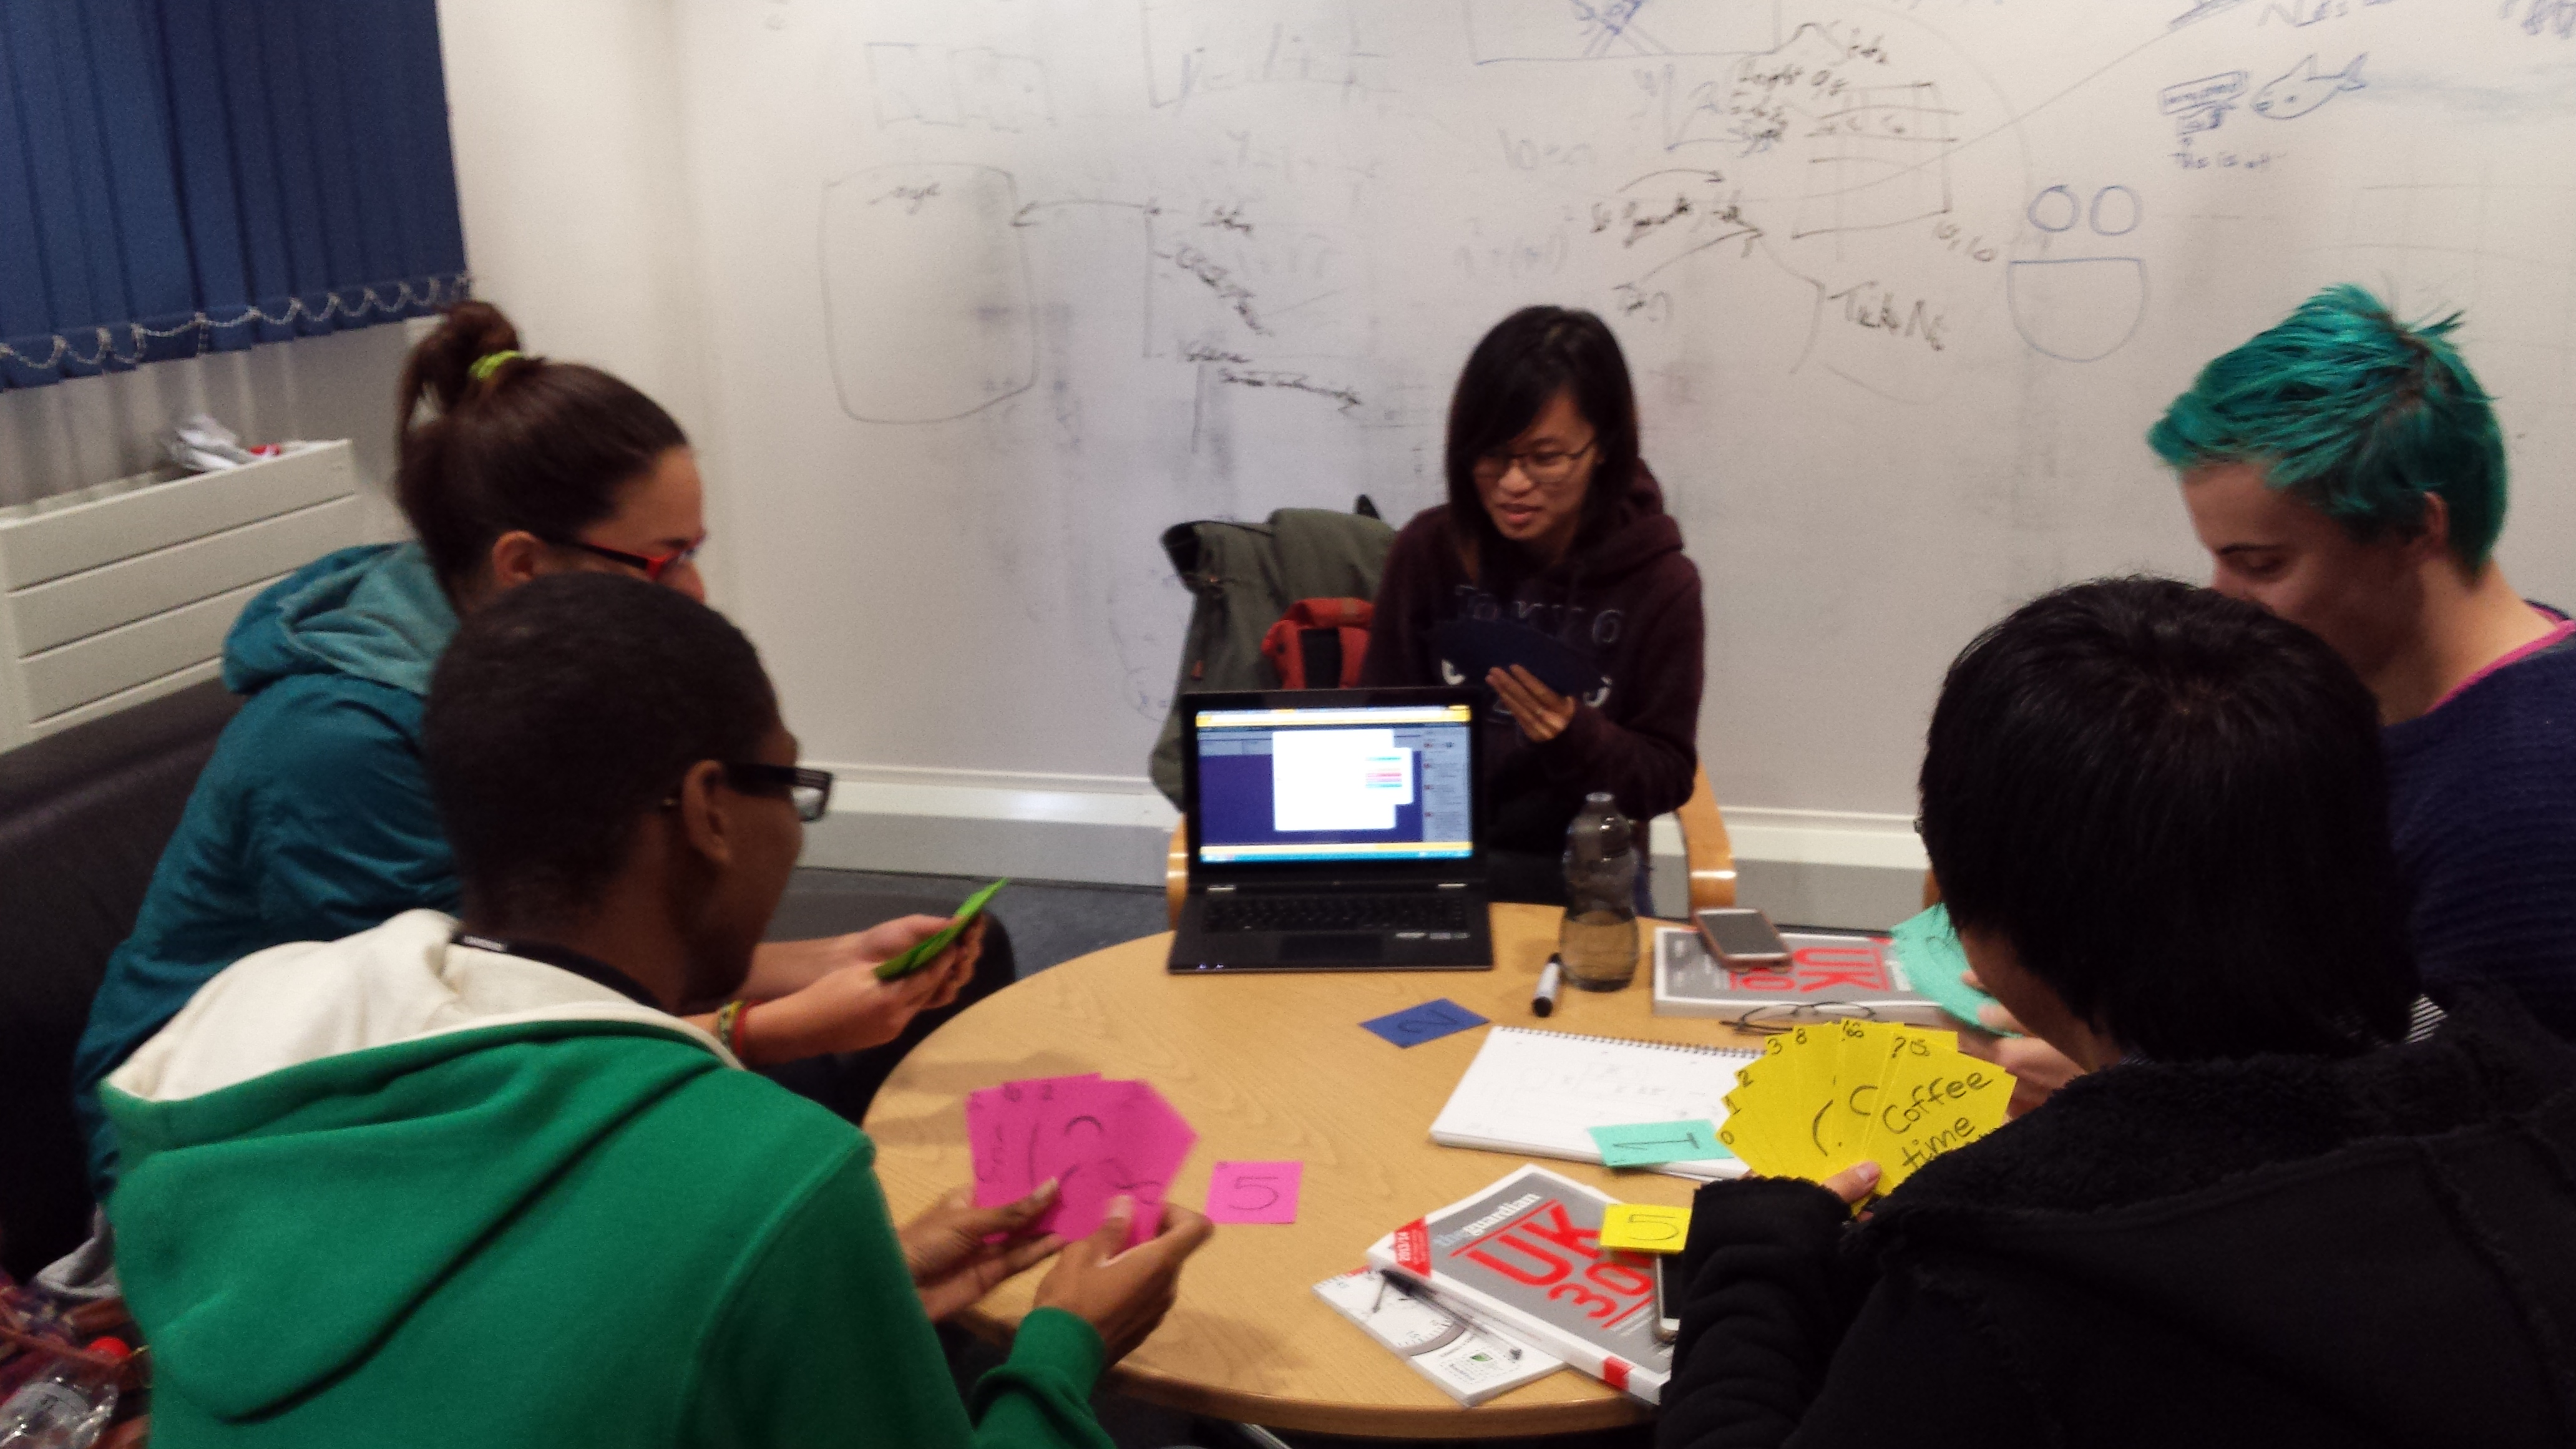
\includegraphics[width=130mm]{estimation.jpg}
\caption{Picture taken during one of the group meeting}
\end{figure}

\subsection{Tools}

To aid the management of the project on a holistic and timely perspective, several tools were used, which will be outlined below.

\subsubsection{Trello}
\begin{figure}[h!]
\centering
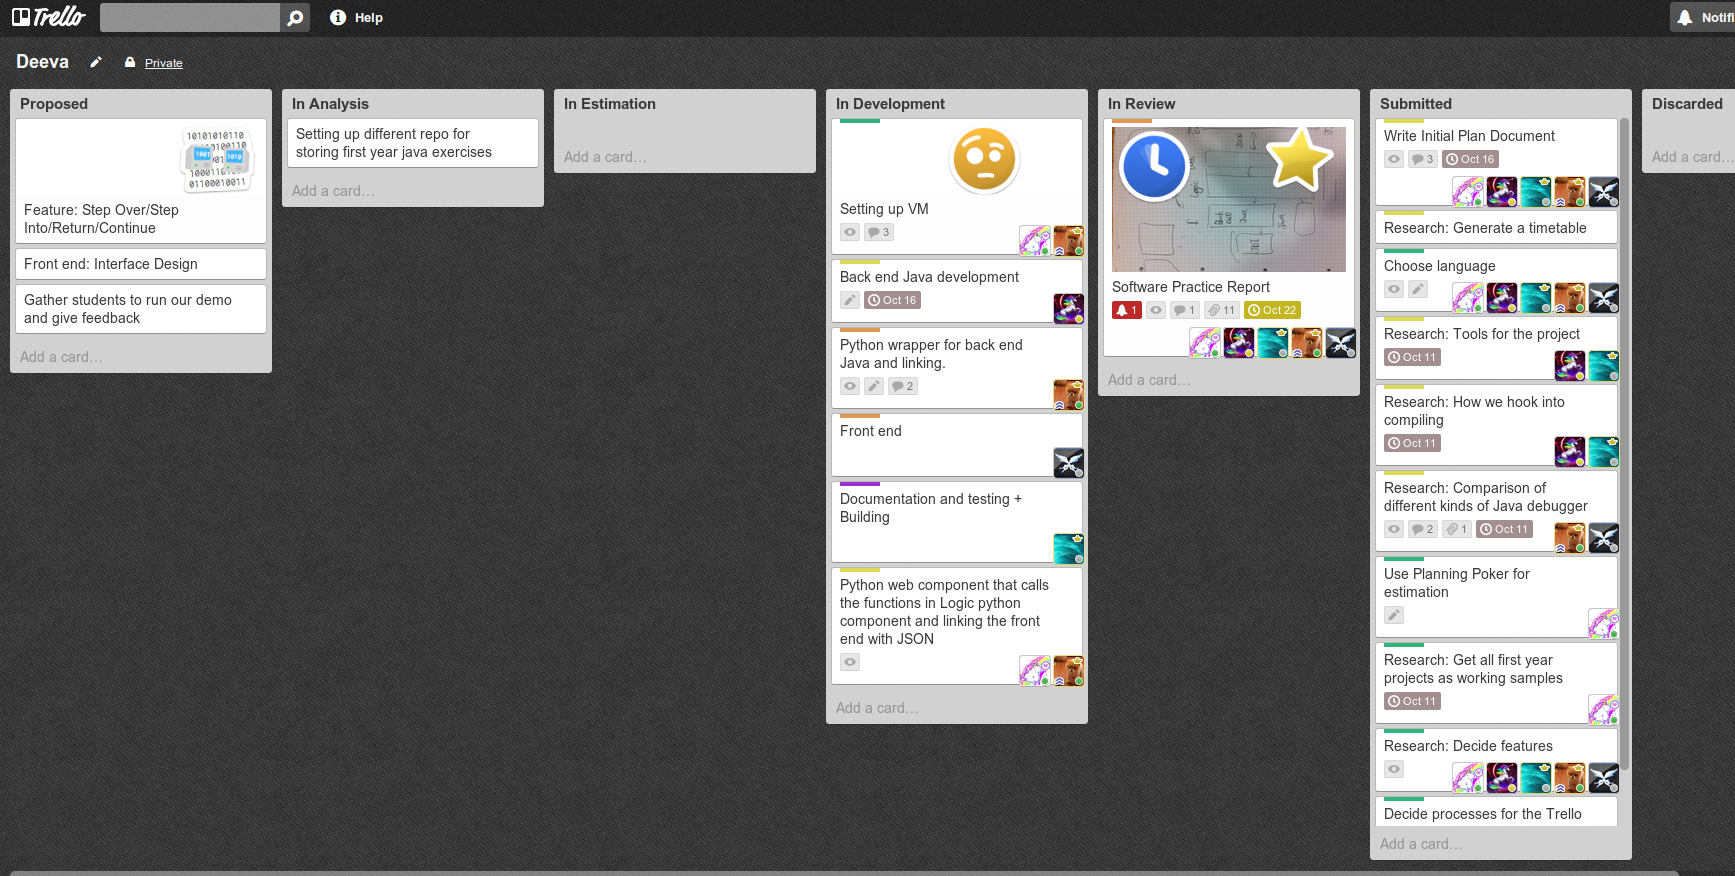
\includegraphics[width=\textwidth]{Trello.png}
\caption{Trello}
\label{fig:Trello}
\end{figure}

We used Trello as our project management tool and as an Information Radiator\footnote{\url{https://www.atlassian.com/wallboards/information-radiators.jsp}}.
It also allows us to track our progress and average velocity.
We decided to use Trello as it fulfills most of the key features required for such a tool: it is easy to use and update, relatively flexible and allows for communications between members without too much interruption.
We decided to use an electronic version as they are a more manageable alternative to physical boards.
We also found it extremely useful when it came to keeping everyone informed on the general progress and keeping all the information in one compact environment.

A Trello board was created for a better project management process.
There are several different swimlanes (see figure~\ref{fig:Trello}) on the board: ``Proposed'', which allows all members to throw in ideas; ``In Analysis'', where people talk about their ideas and have a discussion with group members to see if the story is feasible.
If it is, the card will be then moved to ``In Estimation'' where we would use Planning Poker to assign the story with a complexity points.
Otherwise, the story will be moved to ``Discarded''.
The reason why we want to keep track of what we have discarded is that we might have thought we would not have time for it, but in reality we may have time at the end.
We might want to move it back and reconsider it.
After ``In Estimation'', the card will be assigned to group members with a set due date and be moved into ``In Development'' on the Trello board.
Once the development is complete, the card should be moved into ``In Review''.
This is when we meet as a group and review our code to improve our style and pattern-usage.

\subsubsection{Planning Poker}
\begin{figure}[h!]
\centering
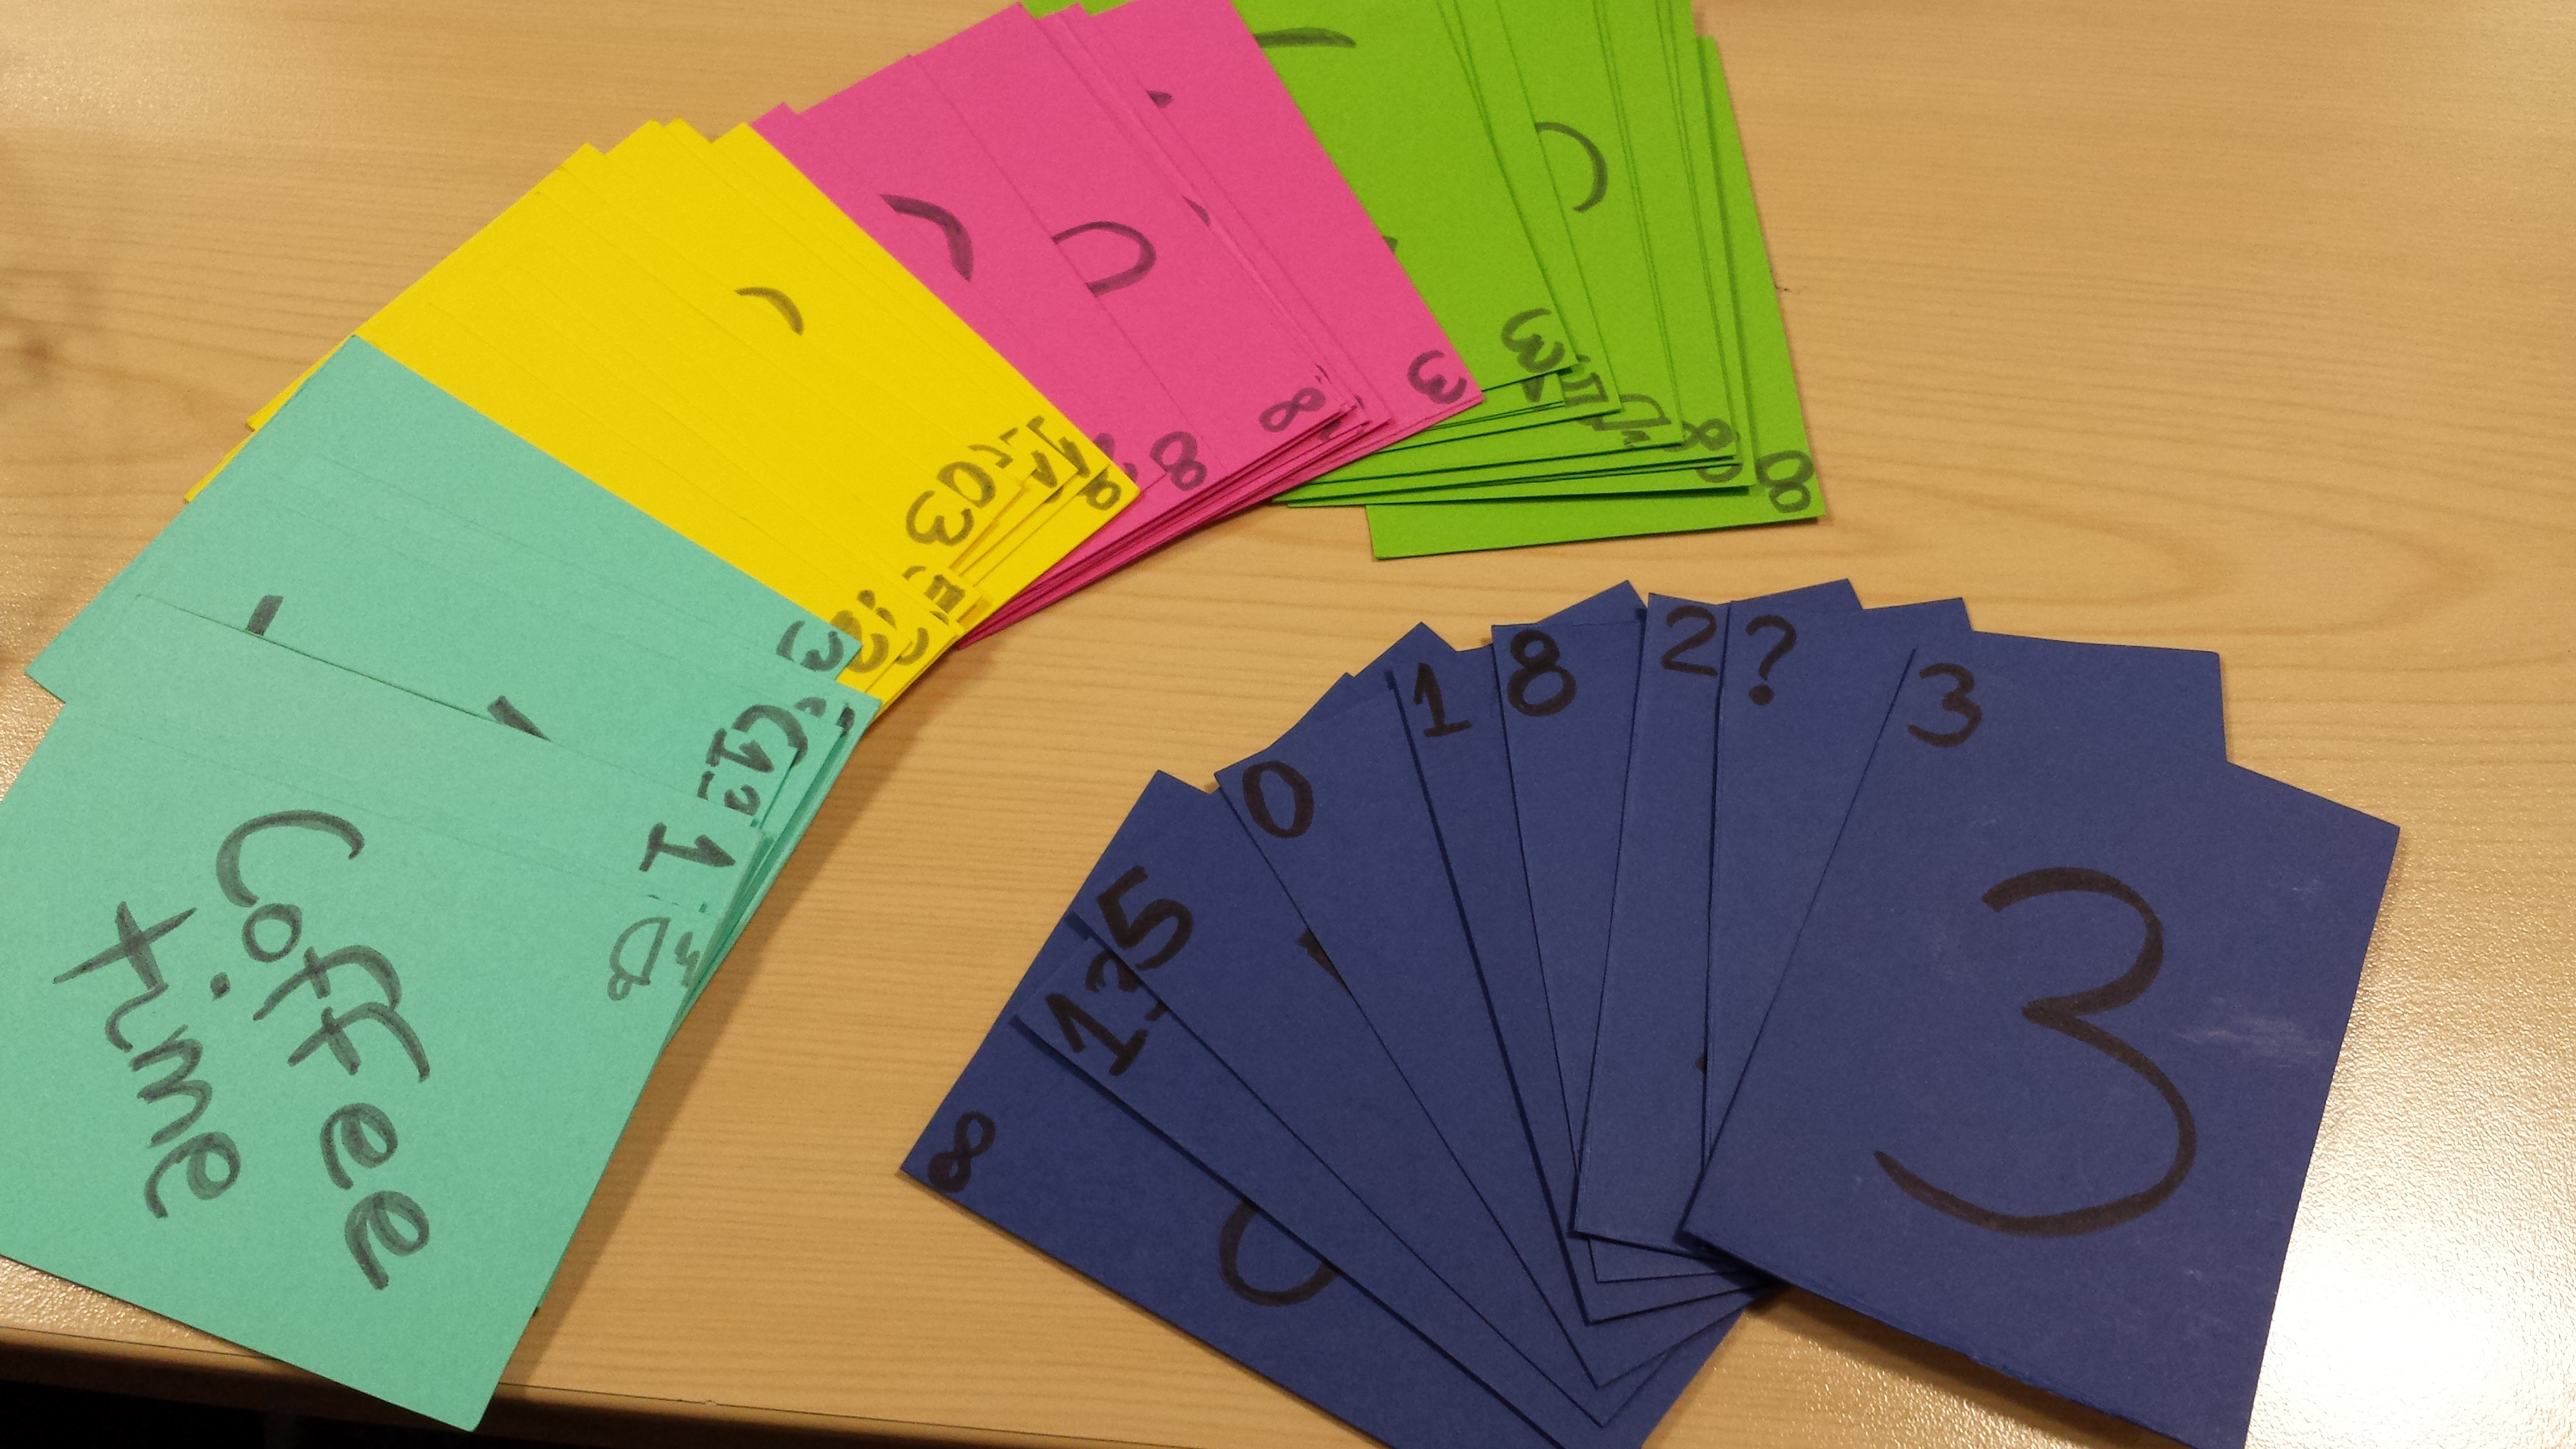
\includegraphics[height=80mm,width=130mm]{planningPokers.jpg}
\caption{Our hand made planning poker cards}
\end{figure}

We are using Planning Poker in order to estimate stories in each cycle of development.
This method is known to avoid anchoring and will produce more accurate, less optimistic story point estimations\footnote{\tt{http://en.wikipedia.org/wiki/Planning\_poker\#Planning\_poker\_benefits}}. This technique takes some time to get used to because initially the story point bared little meaning to us.
As we estimated more tasks, the story points became more meaningful hence the poker game proved to be a very efficient method.

For example, it helped determine when people aren't really talking about the same scope for a certain task.
Frequently we have a task like ``Set up the back end." and one person gives a task a 2 while another gives it an 8.
The first person thinks the task title means ``Write some stubs so the middleware can integrate." while the second thinks it means ``Implement the backend up to the minimal specification.".
So using planing poker has already helped us make sure we're all on the same page.
One of our group members hand-made a set of poker cards just for estimation.
It contains the Fibonacci numbers up to 13 including 0 and infinity - if the task was unfeasible in the time given, as well as ``coffee time'' if we think we needed a break.

\subsubsection{Facebook Group}
Creating a Facebook group proved very efficient for communicating meeting times and general enquiries that were too conversational for Trello.

\subsubsection{Google Docs}
We used Google Docs for collaborative editing on reports, plans and meeting summaries in real time.

\subsubsection{Github}
Github is a hosted source control which somebody else manages and is easily accessible from anywhere and also plays nicely with the hosted Continuous Integration tool we used - Travis CI.
Over the period we worked on this project Github had a few hours of down time but this was easily less than the time it would have taken us to setup and maintain our own source control server.

\subsubsection{Travis CI}
Travis\footnote{\url{http://travis-ci.com/}} is an online continues integration server.
Whenever we push code to the Github server Travis takes the commit then makes and runs our integration tests, if the build fails Travis' emails us.
Ideally the build on Travis should never fail (since we should run the tests ourselves before we commit) but the email notifications proved very useful for problems which only show up on a fresh install or if we made a small commit which ``shouldn't" have broken the build.
Travis' notifications allowed quickly brought bad commits to our attention allowing us to fix or revert them before they became a major problem.
Since Travis has to install all the dependencies each time running the tests can take up to ten minutes.



\subsection{Team Member Contributions}
\subsubsection{Kritaphat Sonsri-in}
\subsubsection{Xueqi Chen}
\subsubsection{Alina Draganescu}
\subsubsection{Felix de Souza}
\subsubsection{Hector Dearman}
Hector worked mostly on the backend implementing Breakpoints and the middle server layer.

\section{Extensions}

\section{Conclusion}


\clearpage
\thispagestyle{empty}
\null\vfill
\begin{center}
\settowidth\longest{``A process cannot be understood by stopping it."}
\parbox{\longest}{%
  \raggedright{%
  ``A process cannot be understood by stopping it." \\
  }
  \raggedright{\emph{First Law of the Mentat -- Dune}}\par%
}
\end{center}
\addcontentsline{toc}{section}{Quote}
\vfill\vfill
\clearpage

\appendix
\section{Initial Plan}
\label{sec:initialplan}
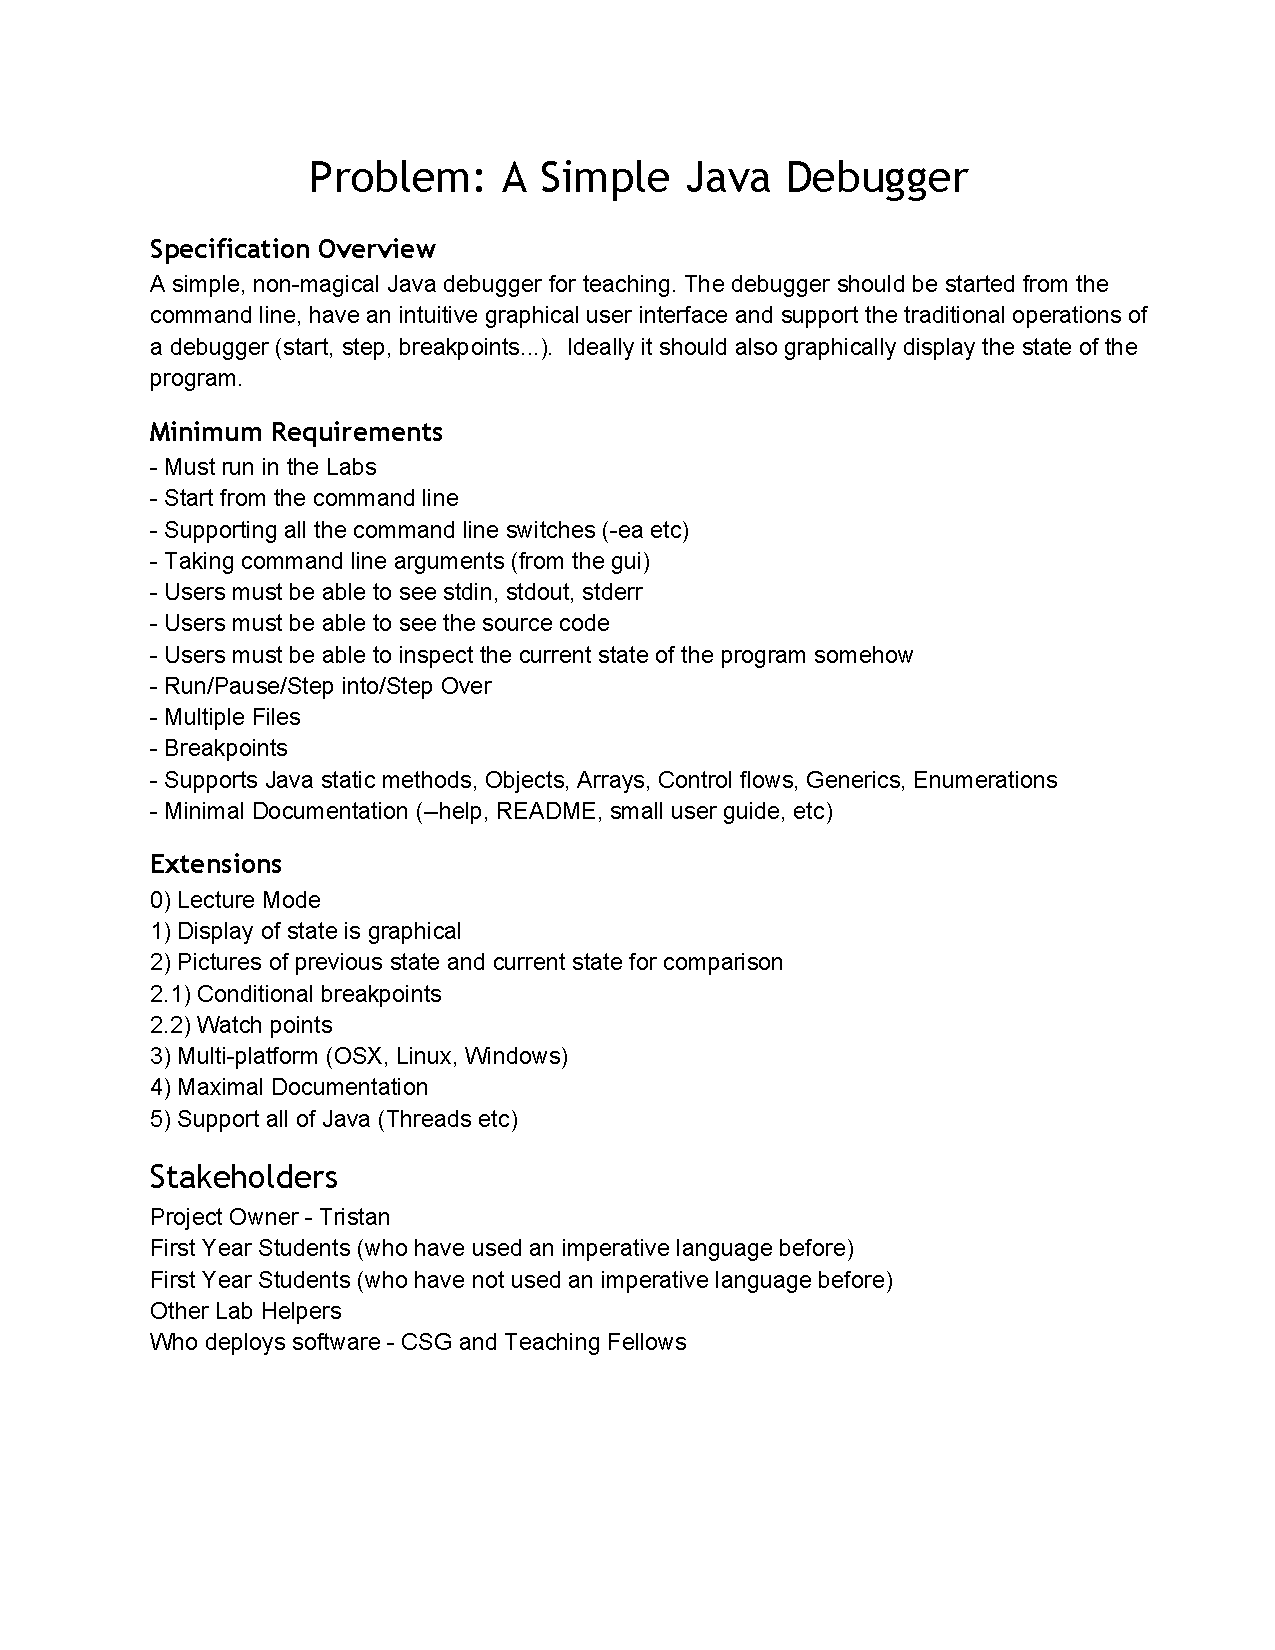
\includepdf[pages={-}, pagecommand={}]{plan.pdf}

\section{Annotated Plan}
\begin{figure}[h!]
\centering
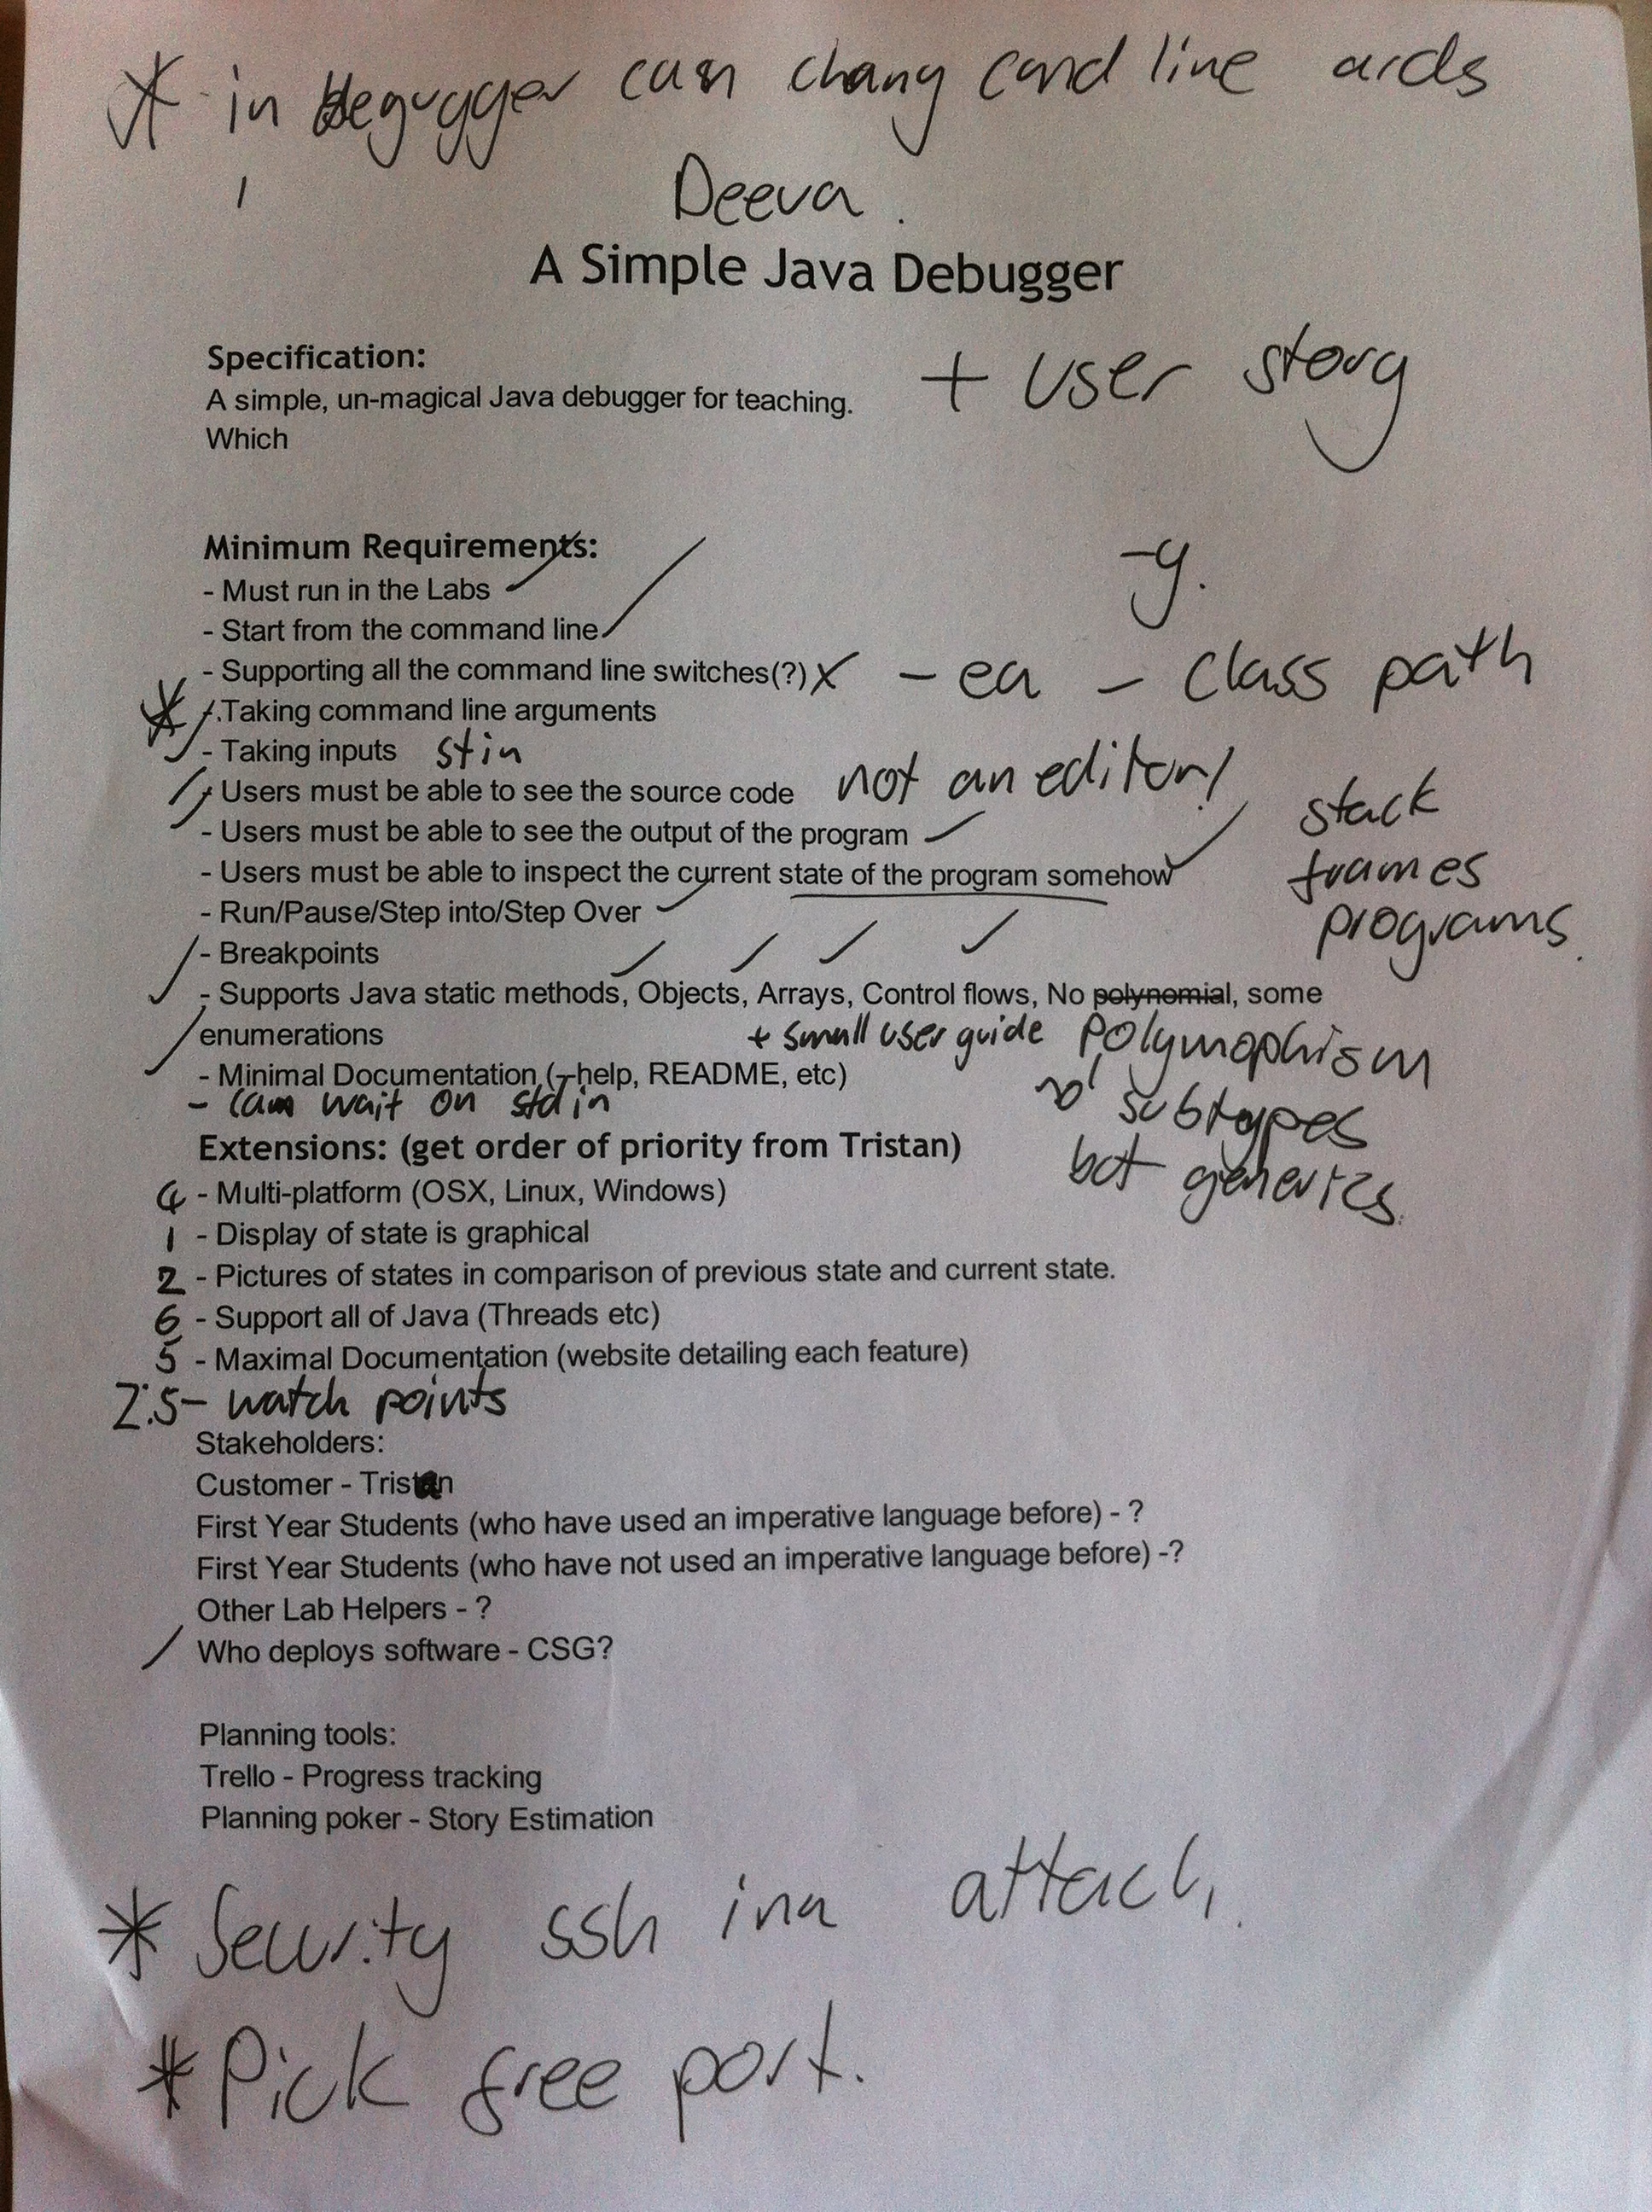
\includegraphics[width=\textwidth]{annotatedreport.jpg}
\caption{An example of notes taken during a meeting with project supervisor.}
\end{figure}

\section{Button Questionnaire}
\label{sec:buttonquestionnaire}
\begin{figure}[h!]
\centering
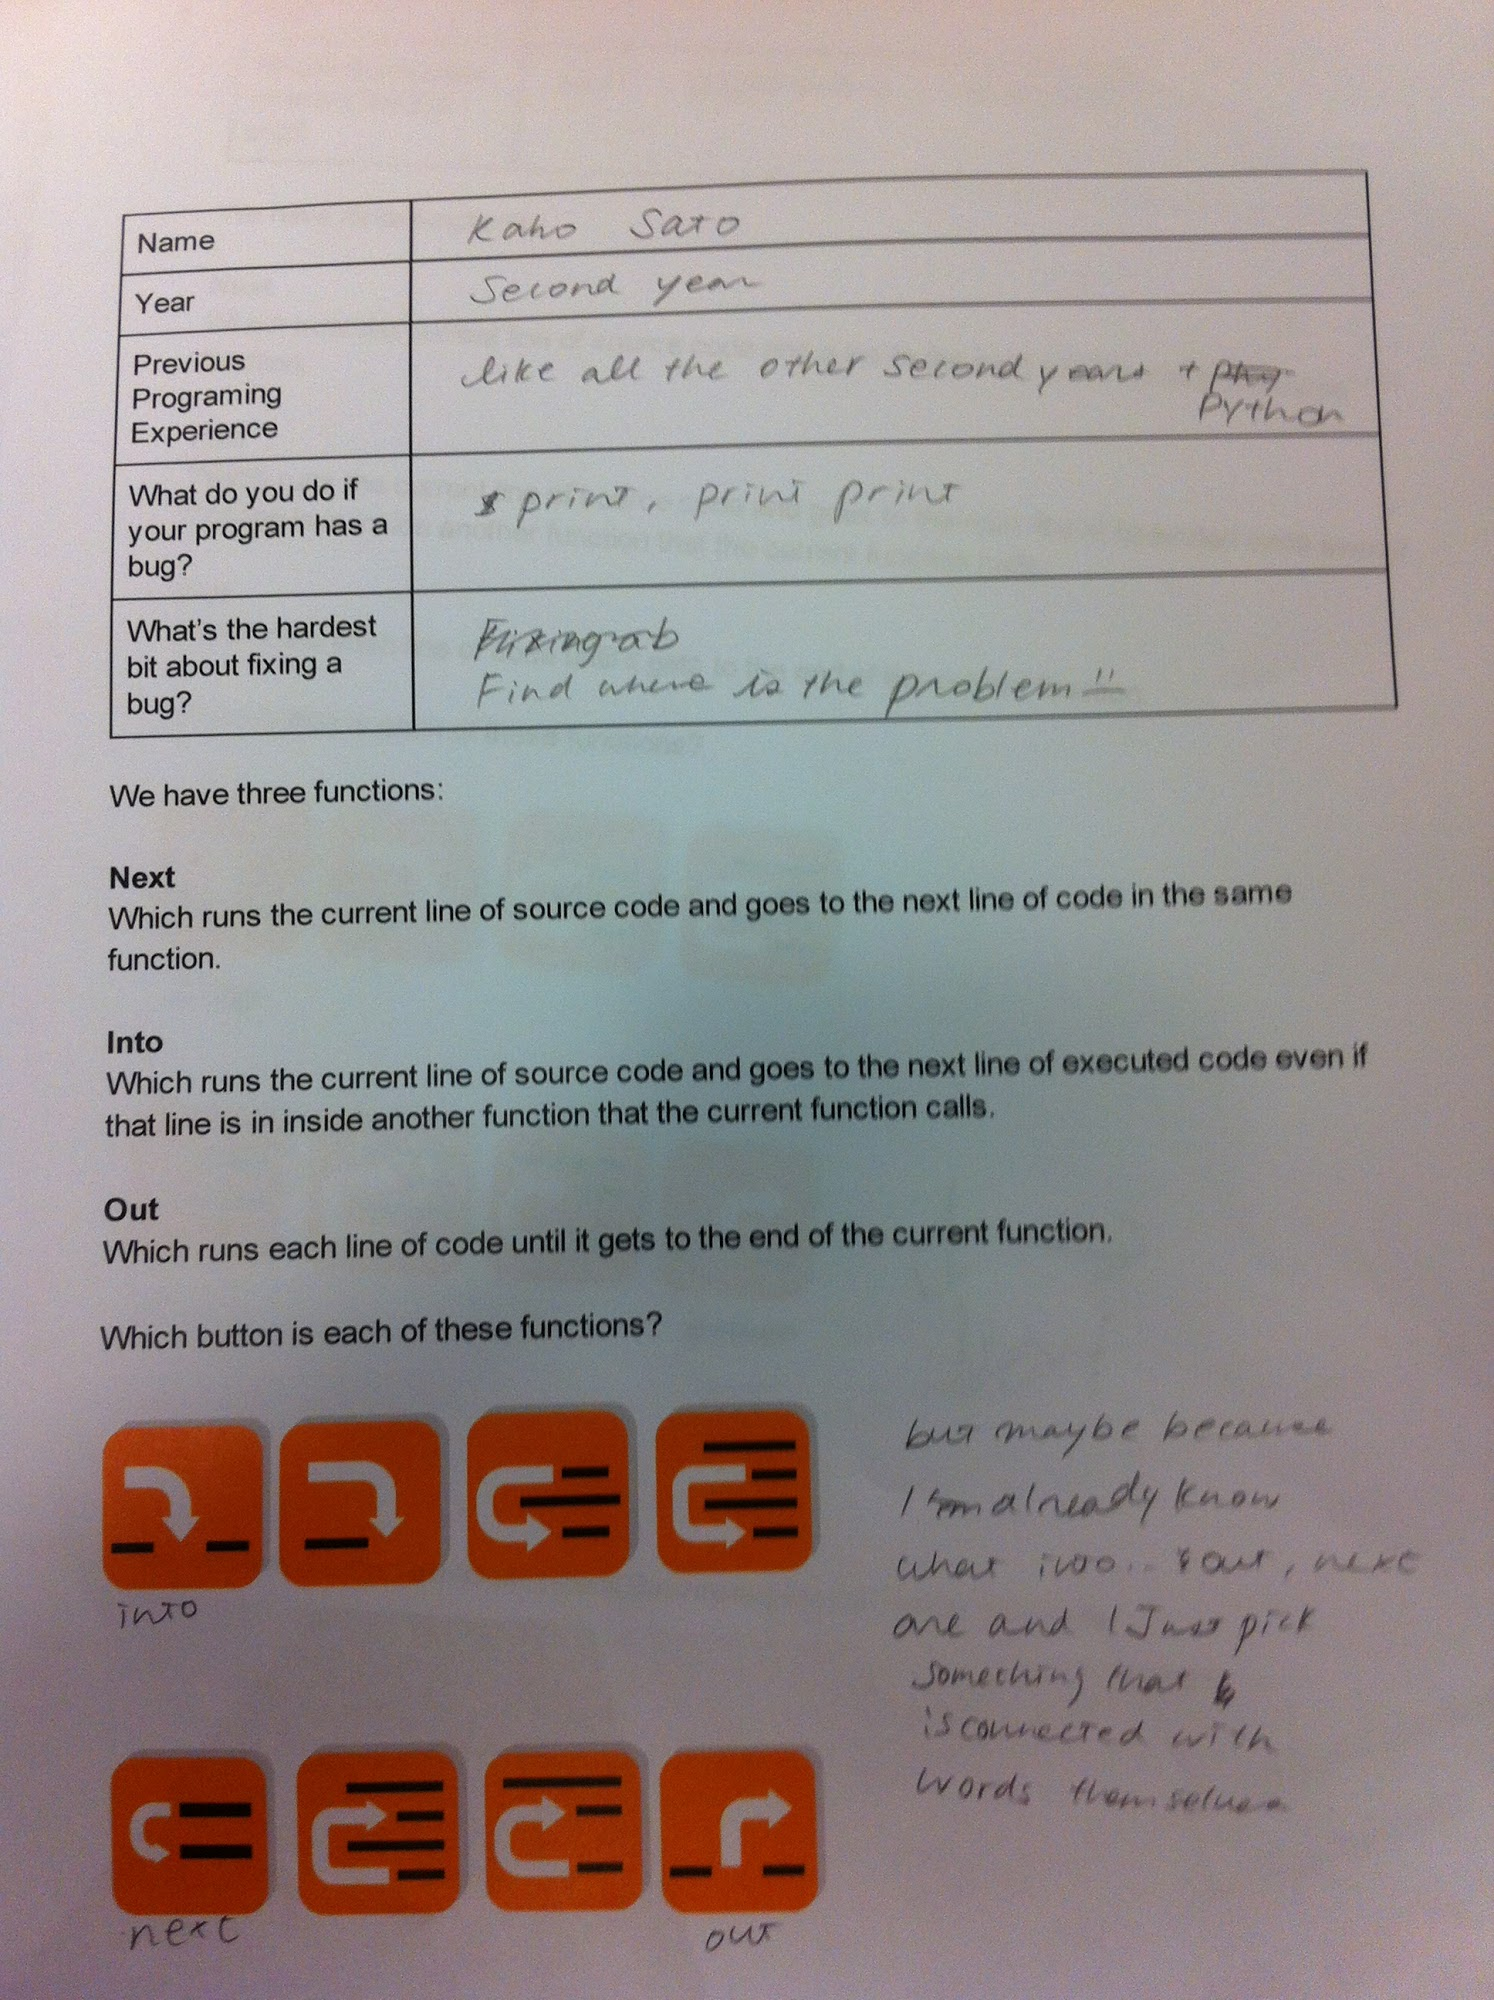
\includegraphics[width=\textwidth]{questionnair2.jpg}
\caption{An example feedback given by a user on our button designs.}
\end{figure}

\section{User Guide}

\begin{thebibliography}{9}

\bibitem{projectproposal}
	Tristan Allwood.
	\emph{Project Proposal: A Java Debugger Suitable for Teaching}.
	\url{https://cate.doc.ic.ac.uk/projects/proposals.cgi?key=2013:1:show-2728}

\bibitem{pythontutor}
	Philip Guo.
	\emph{Python Tutor}.
	\url{http://pythontutor.com/}

\bibitem{saeed09}
	Dehnadi, Saeed, Richard Bornat, and Ray Adams.
	\emph{Meta-analysis of the effect of consistency on success in early learning of programming.}
	PPIG, 2009.

\bibitem{CodeMirror}
	Marijn Haverbeke.
	\emph{CodeMirror}.
	\url{http://codemirror.net/}

\bibitem{blinker}
        Jason Kirtand.
        \emph{Blinker}
        \url{http://pythonhosted.org/blinker/}

\bibitem{jvmti}
        Wikipedia.
        \emph{Java Virtual Machine Tools Interface}
        \url{http://en.wikipedia.org/wiki/Java_Virtual_Machine_Tools_Interface}
        2013

\bibitem{heisenbug}
        Wikipedia.
        \emph{Heisenbug}
        \url{http://en.wikipedia.org/wiki/Heisenbug}
        2013

\bibitem{java_available}
        Java Docs
        \emph{Javadoc: InputStream, available()}
        \url{http://docs.oracle.com/javase/7/docs/api/java/io/InputStream.html#available()}
        2011

\bibitem{NIH}
        Wikipedia.
        \emph{Not invented here}
        \url{http://en.wikipedia.org/wiki/Not_invented_here}
        2013

\bibitem{D3}
        D3 docs.
        \emph{Data-Driven Documents}
        \url{d3js.org}
        2013

\bibitem{NIH}
        Bootstrap docs.
        \emph{Bootstrap}
        \url{http://getbootstrap.com/}
        2013
\end{thebibliography}

\end{document}
